\documentclass[a4paper, 12pt,openany]{book}


\usepackage[a4paper, left=2.5cm, right=2.5cm, top=3cm, bottom=3cm]{geometry}
\usepackage{times}
\usepackage{afterpage}
\usepackage[utf8]{inputenc} %¡¡NO codificar en latin!!
\usepackage[spanish]{babel} % Comenta esta línea si tu memoria es en inglés
\usepackage{url}
%\usepackage[dvipdfm]{graphicx}
\usepackage{graphicx}
\usepackage{caption}
\usepackage{subfigure}
\usepackage{listings}
\usepackage{color}
\usepackage[dvipsnames]{xcolor}
\lstset{ %
	breakatwhitespace=true,
	breaklines=true, 
	stringstyle=\color{BrickRed},
	basicstyle=\ttfamily\small,
	backgroundcolor=\color{white},  % choose the background color. You must add \usepackage{color}
	keywordstyle=\color{RoyalBlue},
	commentstyle=\color{OliveGreen},
	deletekeywords={list},
	otherkeywords={String},
	showspaces=false,               % show spaces adding particular underscores
	showstringspaces=false,         % underline spaces within strings
	showtabs=false,                 % show tabs within strings adding particular underscores          
	tabsize=3,          % sets default tabsize to 2 spaces
	captionpos=b,           % sets the caption-position to bottom
	frame=tb,
}

\graphicspath{ {img/} }
\usepackage{enumitem}
\usepackage{pifont}
\usepackage{amssymb}
\usepackage{float}  %% H para posicionar figuras
\usepackage[nottoc, notlot, notlof, notindex]{tocbibind} %% Opciones de índice
\usepackage[none]{hyphenat}
\usepackage{cite}
\usepackage[pagestyles]{titlesec}
\usepackage{lipsum}
\setcounter{tocdepth}{3} %para que el índice llegue hasta subsubsection
\usepackage[bookmarks = true, colorlinks=true, linkcolor = black, citecolor = black, menucolor = black, urlcolor = blue]{hyperref} %para que los enlaces no aparezcan recuadrados en rojo y cambia los colores de los enlaces
\setcounter{secnumdepth}{3}

\begin{document}

	\begin{titlepage}
		\centering
		
\includegraphics[scale=0.5]{logo_urjc.jpg}
		\vspace{3cm}
		
		\Large
		GRADO EN INGENIERÍA EN TECNOLOGÍA DE LAS TELECOMUNICACIONES
		
		\vspace{0.4cm}
		
		\large
		Curso Académico 2021/2022
		
		\vspace{0.8cm}
		
		Trabajo Fin de Grado
		
		\vspace{2.5cm}		
		\LARGE		
		ROBÓTICA EDUCATIVA CON PYTHON Y MBOT
		
		\vspace{2.5 cm}
		
		\large
		Autor :  Eva García Domingo\\
		Tutor : Jose María Cañas Plaza \\
		\afterpage{\null\newpage}
		\pagestyle{empty}
	\end{titlepage}
	
	%\chapter*{}

\begin{flushright}
	\textit{Dedicado a \\
		mi familia, amigos, pareja mascotas, compañeros de estudios.
\end{flushright}
\afterpage{\null\newpage}


	%\chapter*{Agradecimientos}
\thispagestyle{empty}
\label{cap:agradecimientos}

\begin{flushright}

	\textit{En este Trabajo hay mucho que agradecer}
	
		\vspace{2cm}
	\textit{A la familia, claro. La nativa y la elegida. No hay nadie que me haya aguantado ni apoyado tanto, manteniéndose siempre a la distancia justo necesaria}
	
		\vspace{1cm}
	\textit{A los amigos, tan necesarios para superar todo lo imaginable}
	
	\vspace{1cm}
	\textit{Y a mi tutor, Jose María, por no dejarme por imposible. He aprendido mucho más de lo que buscaba.}
\end{flushright}

\afterpage{\null\newpage}
\pagestyle{empty}
	%
\chapter*{Resumen}


\label{cap:resumen}

Este Trabajo Fin de Grado se fundamenta en una necesidad de enseñar robótica y pensamiento computacional a alumnos y alumnas sin conocimientos previos ni de robótica ni de programación. El objetivo es ofrecer una solución para introducir e interesar a estudiantes en la disciplina, de forma sencilla y efectiva, evitando las dificultades propias de la programación de robots.\\

Con esta finalidad, ofrecemos una plataforma para la programación del robot mBot en Python, creando una capa de aplicación visible al usuario que ocultará toda la funcionalidad de las  comunicaciones con el robot real, que sólo admite programación en Arduino. La característica principal de esta plataforma será la accesibilidad, en herramientas tanto software como hardware, con el objetivo de hacerla lo más accesible posible a la mayor cantidad de estudiantes.\\

Hemos diseñado un curso escolar, fundamentalmente práctico, estructurado en dos partes. Con la primera, utilizamos la plataforma del mBot ofrecida por el fabricante, de programación visual por bloques. Durante la segunda parte del curso utilizaremos la plataforma y API desarrollada en Python, con un lenguaje de texto más cercano a la programación clásica.\\

\afterpage{\null\newpage}
	
	\tableofcontents
	\pagenumbering{arabic}
	\setcounter{page}{1}
	\mainmatter

	\chapter{Introducción}\label{cap:introduccion}

\section{Robótica y tecnologías afines}\label{sec:contextoIntroduccion}
Durante mucho tiempo la robótica ha sido una disciplina muy alejada y poco accesible al público, tanto por su coste económico, como por el difícil acceso a recursos académicos (manuales teóricos o recursos humanos). Esto la ha convertido, en lo que se refiere a una visión popular, en una disciplina de lujo accesible a unos pocos privilegiados económica o académicamente (agencias espaciales, grandes corporaciones, robots súper funcionalea, etc) llegando incluso a ser más cercana a la ciencia ficción que a la ingeniería corriente. No era vista como una disciplina científica cercana a la que poder dedicarse, mucho menos como una asignatura accesible a estudiantes jóvenes o universitarios. \\
Además, el  ``resultado'' de la robótica tampoco era visto como algo real, sino como ciencia ficción o productos de lujo económico. No se concebían los robots como algo adaptable a la vida corriente ni se pensaba en soluciones \textit{robóticas} a problemas reales. A esta visión de la robótica y de los robots ha contribuido en gran medida la literatura y el cine, creando en el imaginario popular robots humanoides indistinguibles de personas reales, completamente independientes y funcionales o inteligencias artificiales utilizadas para viajes espaciales que crecen y se desarrollan al margen de la humanidad.\\

Durante los últimos años, no obstante, se ha observado un cambio de paradigma, impulsado desde el mundo de la ingeniería y el pragmatismo comercial. Los robots han dejado de verse como ``humanos electrónicos'', convirtiéndose poco a poco en una definición más realista, como un proceso electrónico programado para cumplir una o varias funciones interactuando con el medio. Tenemos varios ejemplos de esta nueva definición de robótica:

\begin{description}
	\item [Automatismos.] También llamados \textit{\textbf{bots}}, son un robot sin una capa física que funciona de forma independiente recogiendo datos, procesándolos y respondiendo a ellos de forma \textit{inteligente}. Algunos ejemplos son los aplicativos de \textit{metadata} (muy extendidos) o los conocidos ``chat de ayuda'' en las aplicaciones web (asistentes de ayuda al cliente). Otro ejemplo de uso de estos automatismos son los procesos de seguridad de los vehículos modernos, que se mantienen recogiendo datos del medio  para ofrecer una capa añadida de seguridad frente a posibles errores humanos (velocidad, proximidad y velocidad de otros vehículos, distancias entre carriles, etc).\\
	Una de las características principales de estos \textit{procesos robotizados} es que arrancan sin requerir interacción. Aparte de que una vez funcionando respondan a peticiones o estímulos humanos, no requieren de que se les ``ordene'' encenderse. Siempre pueden apagarse, por motivos obvios de seguridad, pero volverán a arrancar con la misma configuración y, lo más importante, sin necesitar de ningún \textit{reset} o configuración inicial.
	
	\begin{figure}[h]
		\centering
		\begin{subfigure}
			[Seguridad robotizada en un coche]{
			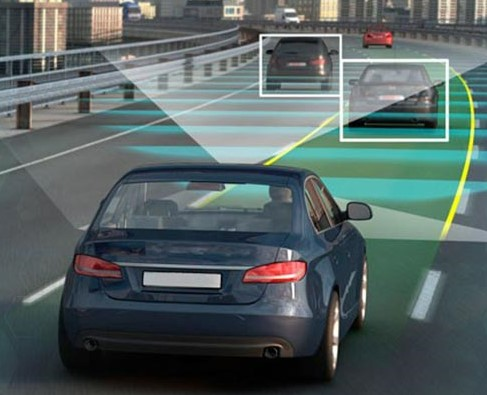
\includegraphics[scale=0.5]{coche.jpg}
			\label{img:coche}
		}
		\end{subfigure}
	\begin{subfigure}
		[Chatbot de ayuda comercial]{
			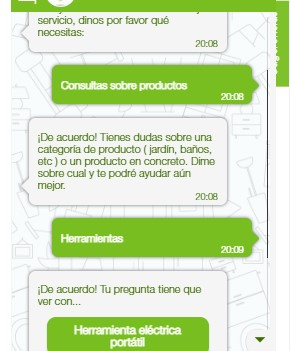
\includegraphics[width=6cm]{chatbot.jpg}
			\label{img:chatbot}
		}
	\end{subfigure}
	\caption{Ejemplos de automatismos}
	\label{img:bots}
	\end{figure}

	\item [Internet Of Things.]\footnote{Internet de las cosas} Muy escuchado, aunque popularmente no se conecte con la robótica. La idea básica del IOT es añadirle conexión a Internet a objetos de uso diario, con los objetivos de:
	\begin{itemize}
		\item Añadir funcionalidades que requieren de conexión online. Por ejemplo, un reloj inteligente con el que poder atender mensajes o llamadas o pagar compras. El usuario interactúa con estas funcionalidades para obtener una respuesta, aunque la aplicación se mantiene funcionando siempre. Es decir, funciona esperando un estímulo al cual responder.
		\item Recoger datos para procesarlos y ofrecer información añadida en función de esos datos. El mismo reloj inteligente recoge datos de sueño, y te muestra la calidad y horas de éste. Con estas funciones no es necesario interactuar sino que están preparadas para recoger datos siempre que estén disponibles y mostrar al usuario los resultados de los procesos que tenga programados.
	\end{itemize}
	El IOT funciona con procesos robotizados, programados para recoger datos de forma automática o responder a estímulos del medio, que siguen las mismas normas antes mencionadas: se mantienen funcionando (siempre que no se les apague expresamente) sin necesidad de configuraciones añadidas; su programación se encarga de ello. Ciertamente, muchos objetos con IOT necesitan de datos iniciales para su puesta en marcha debido a que los datos recogidos son biométricos y necesitan de un contexto inicial para el procesamiento de datos. Podemos ver varios ejemplos de IOT en la figura \ref{img:IOT}.
	\begin{figure}[h]
		\centering
		\begin{subfigure}
			[Información de la calidad del sueño proporcionada por un reloj inteligente] {
			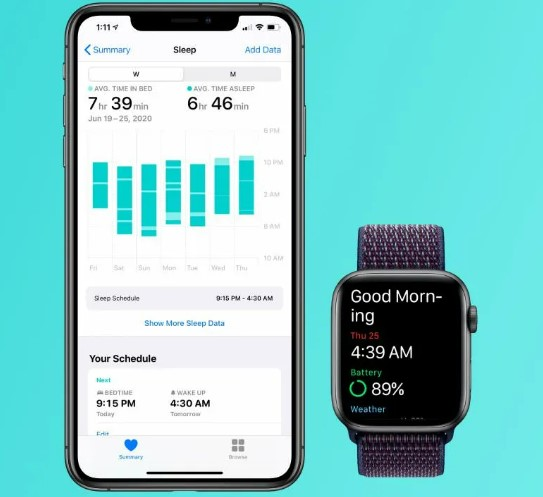
\includegraphics[scale=0.5]{IOT1.jpg}
			\label{img:IOT1}}
		\end{subfigure}
		\begin{subfigure}
			[Báscula inteligente que procesa los datos almacenados] {
			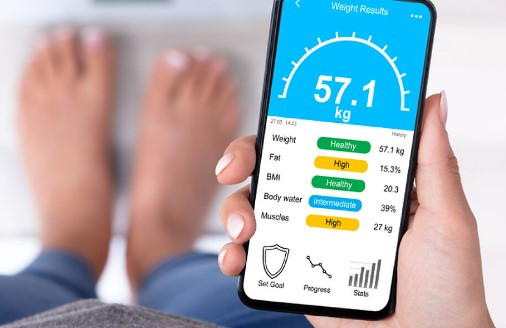
\includegraphics[scale=0.5]{IOT2.jpg}
			\label{img:IOT2}}
		\end{subfigure}
		\newline
		\begin{subfigure}[c]
			[Aplicación conectada a un sensor de glucosa para controlar el nivel de azúcar] {
			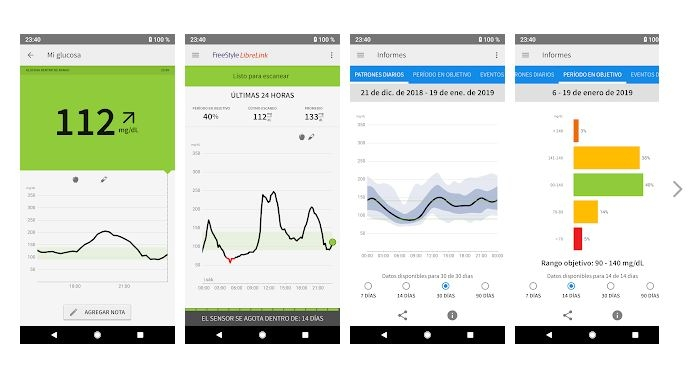
\includegraphics[scale=0.5]{IOT3.jpeg}
			\label{img:IOT3}}
		\end{subfigure}
		\caption{Ejemplos de IOT}
		\label{img:IOT}
	\end{figure}

	\item [Domótica.] Posiblemente la utilidad robótica más extendida a día de hoy. Cada vez más unida al IOT, aunque no lo requiere expresamente. Viene del significado latino de 'casa' y engloba a todo sistema o automatismo diseñado para cumplir una función que facilite una tarea doméstica o le añada funcionalidad. Tenemos sistemas de seguridad, aspiradores, electrodomésticos que se comportan diferente dependiendo de las circunstancias (cantidad de agua de una lavadora, o temperatura de un frigorífico), control de luces con aplicaciones móviles (tanto con Internet como sin él), controles de accesos, etc. Todo esto son procesos robotizados (robots al fin y al cabo) que utilizan información del medio para reaccionar de una u otra manera. Esta información puede provenir de sensores (la lavadora o el frigorífico) o recibirla del usuario/a (apagar o encender las luces, la TV o la alarma). En la figura \ref{img:domotica} tenemos ejemplos de aplicaciones domóticas.
	\begin{figure}[h]
		\centering
		\begin{subfigure}
			[Robot aspirador] {
				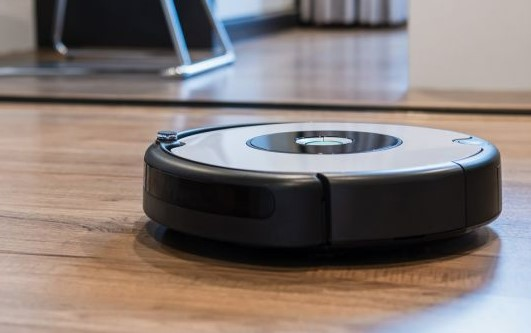
\includegraphics[scale=0.5]{domotica1.jpg}
				\label{img:domo1}}
		\end{subfigure}
		\begin{subfigure}
			[Elementos para control inteligente de luces] {
				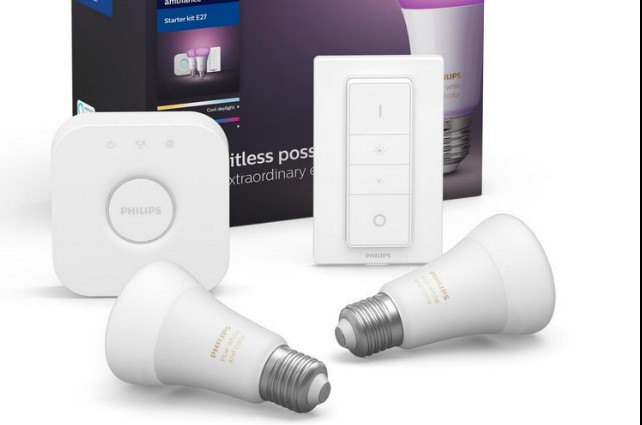
\includegraphics[scale=0.5]{domotica2.jpg}
				\label{img:domo2}}
		\end{subfigure}
		\caption{Ejemplos de domotica}
		\label{img:domotica}
	\end{figure}
	\item [Inteligencia Artificial.] Uno de los grandes trabajos respecto al cambio de visión de la robótica ha sido conseguir cambiar el ideario de Inteligencia Artificial y de separarlo del concepto de robot. Lejos del concepto que tradicionalmente se tenía de Inteligencia Artificial (como hemos comentado, en parte culpa de la ciencia ficción, por ejemplo el robot M.A.D.R.E. de la pelicula \textit{Alien}), podemos encontrar inteligencias artificiales habitualmente en nuestro día a día. Por ejemplo, los asistentes virtuales de diferentes fabricantes (Google, Amazon o Apple) aprenden del medio en mayor o menor medida y son capaces de buscar una respuesta que no tienen pre-programada (un ejemplo de estas IA está en la figura \ref{img:alexa}), o los programas de procesamiento de \textit{big data} que se realimentan con los datos que recogen y de sus propios resultados para afinar esos mismos algoritmos de procesamiento.
	\begin{figure}[h]
		\centering
		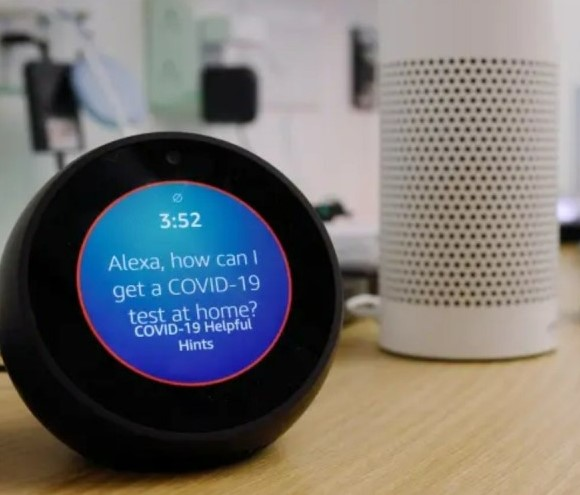
\includegraphics[scale=0.5]{alexa.jpg}
		\caption{Inteligencia Artificial}
		\label{img:alexa}
	\end{figure}
	
	\item [Juguetes robots] Finalmente, llegamos a la aplicación más reconocible como ``robot'' propiamente dicho, también muy lucrativa. La robótica ha tenido un gran impulso en el ocio, creándose diferentes juguetes tanto para niños como para adultos. Se han convertido de ser un juguete de élite a tener variedad de opciones, con diversas funcionalidades, y accesibles a más variedad de costes. Esta accesibilidad de la robótica en el ocio ha contribuido en gran medida a esa transformación de la robótica y a incluirla en nuestras vidas, dando lugar a muchas otras aplicaciones. Una aplicación robótica que empieza siendo un juguete, puede convertirse en algo mucho más práctico e importante. Por ejemplo, los drones (en la figura \ref{img:drones}), que tienen cada vez más utilidades diferentes.
	
	\begin{figure}[h]
		\centering
		\begin{subfigure}
			[Drone teledirigido orientado al ocio grabando deporte] {
				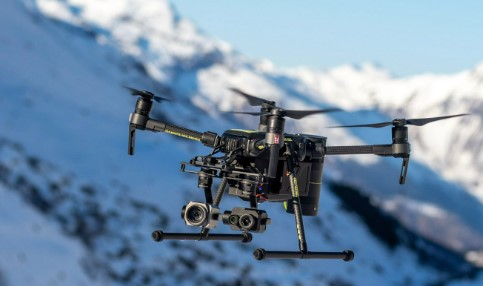
\includegraphics[width=0.33\textwidth]{droneski.jpg}
				\label{img:drone1}}
		\end{subfigure}
		\begin{subfigure}
			[Drone de ayuda humanitaria] {
				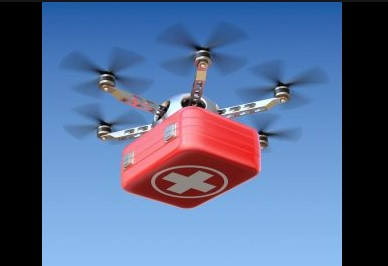
\includegraphics[width=0.33\textwidth]{dronerescate.jpg}
				\label{img:drone2}}
		\end{subfigure}
		\caption{Diferentes ejemplos de uso para un mismo tipo de robot}
		\label{img:drones}
	\end{figure}
	
	
	En cuanto a este Trabajo Fin de Grado, esta aplicación es la que más nos interesa.
\end{description}

\section{Robótica Educativa}


Estos cambios por parte de la industria y avances por parte de la ingeniería han contribuido a acercar la robótica a las personas de a pie, sobre todo a las generaciones más jóvenes, facilitando el acceso a recursos con los que aprender y creando un interés por ello. Es muy notable el abaratamiento de los diversos componentes, así como de los productos finales, y la introducción de esta disciplina en los diferentes niveles educativos (sobre todo en estudios universitarios). El hecho que más gente tenga acceso a los recursos necesarios, y tenga desde joven los conceptos inculcados, contribuye a aumentar las aplicaciones prácticas en todos los ámbitos, y a resolver problemas en los que anteriormente, al no ser una disciplina extendida, quizá nadie había reparado. \\

Sin embargo, y a pesar de todo este trabajo realizado y todo lo conseguido, aún queda mucho por trabajar. El principal problema para que una persona se ponga a aprender cómo programar un \textit{comportamiento robótico} es que debe aprenderlo desde cero, sin haber tenido un aprendizaje progresivo como con el resto de enseñanzas. La Matemática, la Física o la Química, se enseña con niveles progresivos de dificultad, desde edades muy tempranas con las metodologías y conceptos ampliamente discutidos y formulados, para poder llegar a aplicaciones más avanzadas. Nadie espera que una persona sin conocimiento ninguno de estas materias, arranque  un curso de, por ejemplo, Cálculo Diferencial, Matemática Discreta o Teoría Gravitatoria. Es decir, se \textit{educa} al cerebro desde el principio, cuando más capacidad de aprendizaje se tiene, para adaptarse a nuevos conceptos y poder aprenderlos gradualmente. \\
\par Con la robótica y el pensamiento computacional no se ha seguido ese orden lógico. La mayoría de los estudiantes que aprenden Programación, Computación o Algoritmia lo hacen a edades más avanzadas, ya sea por su cuenta o con educación reglada. Si esta educación comenzara, como otras disciplinas, con los alumnos y alumnas siendo mucho más jóvenes y avanzara con ellos durante las siguientes etapas educativas, se conseguiría que llegaran a las más avanzadas mucho más preparados. Además despertaría en muchos más estudiantes la curiosidad por estas carreras, tanto profesional como educativamente.\\

Para responder a esta necesidad han surgido varios entornos de robótica educativa orientada a niños y niñas. Los principios fundamentales de todos ellos son parecidos. Buscan la simplicidad, evitando complicados lenguajes de programación, y crear una plataforma visual y llamativa con la que llamar la atención de los niños. Algunos de ellos son:
\begin{description}
	\item [OpenRoberta]\cite{Roberta} Cuenta con la ventaja de ser una herramienta completamente \textit{online}, con capacidad de almacenamiento en la nube para guardar los avances. La programación de los robot se realiza en un lenguaje visual, sin sintaxis. La característica principal de esta herramienta es la posibilidad de programar algunos robots de forma \textit{simulada}, además del robot real. Así es posible probar un ejercicio mucho más rápidamente que con el robot real, o incluso programar comportamientos sin tener un robot disponible. Además, tiene disponibles varios robots de diferentes fabricantes basados en diferentes placas base (Arduino o Java, por ejemplo). 	
	\begin{figure}[h]
		\centering
		\includegraphics[scale=0.4]{RobertaSimulado.jpg}
		\caption{Entorno simulado de OpenRoberta}
		\label{img:roberta}
	\end{figure}
	
	\item [Lego Boost]\cite{Lego} La famosa empresa de juegos de bloques de construcción tiene varios sets para la construcción de robots orientados a diferentes edades. El robot se programa con una aplicación para dispositivos móviles, y no usa un lenguaje sino bloques pictográficos con los que programar los diferentes bloques, lo que lo hace disponible para niños y niñas muy pequeños. Otra ventaja es que es compatible con el resto de bloques de construcción de la marca, por lo que se puede construir un robot personalizado.
	\begin{figure}[h]
		\centering
		
\includegraphics[scale=0.4]{lego.jpg}
		\caption{Robots con el kit de Lego}
		\label{img:lego}
	\end{figure}
	
	\item [Kibotics]\cite{kibotics} Desarrollada por JdeRobot, está orientada a la robótica educativa a todos los niveles. Ofrece una plataforma donde programar robots, tanto reales como simulados, en Python y Scratch, y cursos en ambos lenguajes para alumnos de diferentes edades. Al disponer de un entorno de programación simulada, no es necesario tener un robot físico para los cursos. 
	\begin{figure}[h]
		\centering
		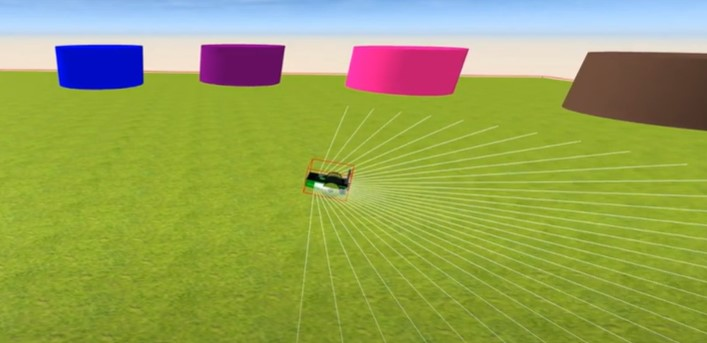
\includegraphics[scale=0.6]{kibotics.jpg}
		\caption{Ejercicio de robótica simulada de un curso de Kibotics}
		\label{img:kibotics}
	\end{figure}
	\item [mBlock]\cite{mblock} Desarrollado por Makeblock \cite{makeblock}, es una de las plataformas para programación de robots educativos más extendida. Es una plataforma, con versiones tanto \textit{online} como instalables para dispositivos móviles y PC, que utiliza el lenguaje de programación para niños Scratch. Contiene los módulos de programación para robots de Makeblock y placas Arduino (puede verse en la figura \ref{img:mblockplacas}).
	
	\begin{figure}[h]
		\centering
		\begin{subfigure}
			[Versión online de mBlock] {
				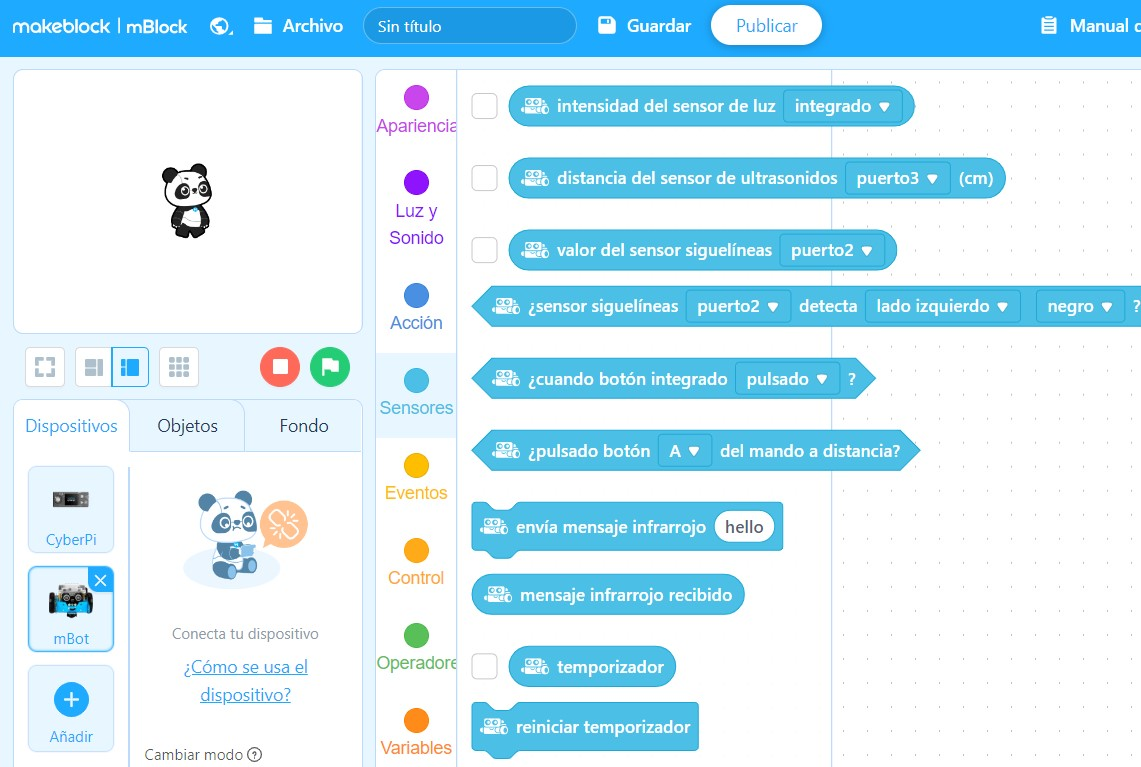
\includegraphics[width=0.6\textwidth]{mblockweb.jpg}
				\label{img:mblockonline}
			}
		\end{subfigure}
		\begin{subfigure}
			[Placas base y robots disponibles en mBlock] {
				\includegraphics[scale=0.7]{mblockPlacas.png}
				\label{img:mblockplacas}
			}
		\end{subfigure}
		\caption{mBlock}		
	\end{figure}

	
\end{description}
\vspace{2cm}
\par Con la idea de introducir en la robótica a niños y jóvenes como principal foco de atención, el propósito de este Trabajo Fin de Grado es ofrecer una propuesta para la enseñanza de robótica y programación a alumnos y alumnas sin conocimientos previos, tanto de Educación Primaria como Secundaria. Para ello se ha utilizado un robot educativo llamado mBot, del fabricante Makeblock \cite{makeblock}, que cumple los requisitos de simplicidad y accesibilidad que requiere el trabajar con niños y niñas. Está especialmente preparado para la enseñanza sin dejar de ser un \textit{juguete}, ya que buscamos despertar el interés y convencer de la facilidad de una disciplina a menudo vista como especialmente complicada y aburrida.

Este proyecto estará compuesto de dos partes. La primera será la creación de una manera sencilla de programar el mBot en el lenguaje de programación Python, siendo éste mucho más sencillo que el lenguaje nativo de la placa base del robot. Se explicará el proceso seguido para desarrollar esta solución, poniendo énfasis en detallar los pasos necesarios para replicarlo, utilizarlo en clases reales con alumnos e incluso ampliarlo. En la segunda parte encontraremos una propuesta completa de uso práctico de esta plataforma, con ejercicios detallados y soluciones de referencia, aumentando el nivel de dificultad progresivamente y con objetivos conceptuales claramente marcados.

Obtendremos así una forma para enseñar de forma accesible y fácil conceptos complejos como algoritmia, programación o metodologías de desarrollo de Software sin necesidad de explicaciones teóricas y poco adaptadas a edades alrededor de los 7-15 años.


\section{Antecedentes}\label{sec:antecedentes}

Dentro de la Universidad Rey Juan Carlos, la organización de software abierto para robótica JdeRobot y particularmente el proyecto PyBoKids \cite{JdeRobot} han servido de antecedente ideológico a este Trabajo Fin de Grado. Ofrecen recursos para robótica educativa, teniendo en cuenta diferentes robot, diferentes plataformas y orientado a varios rangos de edades pre-universitarias.\\

En este Trabajo Fin de Grado hemos tomado del proyecto PyBoKids el propósito educativo, y el concepto de \textit{middleware entre el estudiante y el robot}. Hemos contado como base con la experiencia de un curso escolar de clases extracurriculares de robótica con alumnos de Educación Primaria realizado en el Colegio Nuestra Señora de Rihondo, en Alcorcón. Se comprobó la efectividad del lenguaje Scratch para la enseñanza de robótica y el desarrollo del pensamiento computacional. También se comprobaron las necesidades y limitaciones existentes en caso de querer continuar el curso con un lenguaje textual. De ahí salió la necesidad de una solución educativa sencilla, lo más accesible posible en cuanto a herramientas y conceptos, y con objetivos marcados y preparados para que cualquiera pueda utilizarlos.



	%cada vez que quieras un capitulo nuevo, 
	%descomentarlo y crear el archivo .tex	
	\chapter{Objetivos}
\label{cap:objetivos}
En este capítulo explicaremos los objetivos de este Trabajo Fin de Grado, así como la intencionalidad de ellos y la metología para llevarlos a cabo.
\section{Objetivos}\label{sec:objetivos}
Como se ha adelantado en la Introducción, el carácter principal de este Trabajo Fin de Grado es educacional. Abordaremos dos objetivos complementarios, explicados a continuación. 

\begin{enumerate}
	\item \textit{Diseñar y desarrollar una infraestructura para la programación en Python de un robot basado en Arduino}. Desarrollaremos una biblioteca en Python que utilizar para programar el robot mBot, basado en una placa base de Arduino, con el fin de dar una opción de lenguaje de texto sencilla. También se trabajará en un programa en Arduino que se grabará en la placa base del robot, el cual ofrecerá la comunicación necesaria con la biblioteca de Python. Así, se podrán programar los sensores y actuadores del robot con funciones en Python, cuya lógica estará en esta biblioteca y de la cual no tendrán que preocuparse los alumnos. La solución funcionará en un robot mBot conectado por cable USB al ordenador del estudiante.
	
	\item \textit{Crear una propuesta educativa completa, basada en Scratch y Python, y escalonada según dificultad}. Ofreceremos una propuesta educativa para un curso escolar, orientada según niveles de dificultad y con objetivos docentes detallados. Para ello crearemos diferentes ejercicios prácticos de robótica utilizando el robot educacional mBot, describiendo los objetivos conceptuales que se persiguen. El orden temporal de estos ejercicios estará fijado para de un aprendizaje gradual de programación. Este curso estará orientado a Educación Primaria o Secundaria principalmente (alumnos y alumnas sin conocimientos previos de programación). Para esta propuesta utilizaremos tanto el lenguaje Scratch de programación por bloques, proporcionado por el fabricante, como nuestro \textit{middleware} en Python, como segunda parte avanzada.
\end{enumerate}


\section{Requisitos}\label{sec:requisitos}
Los requisitos que se han marcado para cumplir estos objetivos son los siguientes:
\begin{enumerate}
	\item La plataforma a desarrollar deberá ejecutarse en el lenguaje de programación Python, y el robot educativo mBot podrá programarse en este lenguaje.
	\item Esta plataforma contendrá en una biblioteca los métodos necesarios para empaquetar la lógica de los sensores y actuadores del robot, haciendo esta lógica invisible al usuario.
	\item A bordo del robot habrá asociada una biblioteca de Arduino, desarrollada para establecer una comunicación exitosa entre el robot y la biblioteca Python. Esta biblioteca Arduino deberá poder grabarse en el robot y no tener que cambiarse cada vez que se quiera hacer un programa nuevo para el mBot.
	\item Los ejercicios y prácticas educativas se diseñarán para utilizar el robot mBot y sus periféricos, así como la plataforma de programación del fabricante y la desarrollada en este Trabajo Fin de Grado.
	\item Los contenidos educativos serán una guía de programación y de robótica, y tendrán unos objetivos a corto, medio y largo plazo (por ejercicio, por bloque de lenguaje y por curso). Por edad de los alumnos, podría darse el caso de no poder completar la parte de programación textual; en este caso se orientará el curso para avanzar todo lo posible en la parte de programación visual.  
\end{enumerate}

\section{Metodología y Plan de trabajo}\label{sec:metologia}
Este Trabajo Fin de Grado tiene como punto de arranque la enseñanza de Robótica Educativa durante un curso escolar de clases de robótica a alumnos de Educación Primaria. Con esta base y este conocimiento adquirido, se fijaron los objetivos y sus requisitos para ampliar la propuesta educativa utilizada.\\
Para cumplir estos objetivos, se ha trabajado manteniendo un ciclo semanal de reuniones telemáticas con el tutor, donde se comentaban: avances realizados con respecto a los hitos marcados la semana anterior, problemas encontrados, ideas de trabajo, y nuevos hitos para trabajar durante la semana. Se ha utilizado \textit{Git} como sistema de control de versiones para el código y \textit{GitHub} como repositorio online de almacenamiento del proyecto. Este repositorio está públicamente accesible\footnote{\href{https://github.com/RoboticsLabURJC/2017-tfg-eva_garcia}{https://github.com/RoboticsLabURJC/2017-tfg-eva\_garcia}}.\\
El plan de trabajo para el cumplimiento ha sido el siguiente:
\begin{enumerate}
	\item Familiarización con el entorno robótico de Arduino: uso del robot mBot con el lenguaje nativo de la placa base para entender el funcionamiento de los actuadores y sensores (valores de entrada y salida) y su comunicación con la placa base, además de familiarización con el lenguaje en sí. 
	\item Comunicación ``robótica'' básica entre Python en el PC y Arduino en el robot, a la que ir añadiendo los periféricos del robot.
	\item Diseño de un sistema de mensajes estandarizados para el desarrollo de ambas bibliotecas Python y Arduino con el que poder establecer una comunicación exitosa entre PC y robot.
	\item Desarrollo de ambas bibliotecas con el diseño anterior y diseño de ejercicios en Python utilizando éstas.
	\item Adaptación de los ejercicios realizados durante el curso escolar a la nueva plataforma.
\end{enumerate}
	\chapter{Infraestructura}
\label{cap:infra}

En este capítulo describiremos la infraestructura utilizada, tanto software como hardware, detallando los pasos a seguir si se desea emular. En caso de que algún componente haya sido elegido entre otros de igual aplicación, expondremos las razones de la elección.


\section{Entorno}\label{sec:entorno}
Teniendo el cuenta el carácter educativo de este Trabajo, y su pretendida aplicación en estudiantes de Educación Primaria, se ha elegido el sistema operativo Windows, un entorno conocido, amigable y fácilmente accesible, para instalar y utilizar las diferentes herramientas software. \\
Tradicionalmente, cuando se hablaba de programación y especialmente de programación robótica, siempre se ha utilizado el sistema operativo Linux. Éste daba la posibilidad de instalar todos los paquetes de lenguajes de programación y entornos, mientras que Windows era especialmente cerrado en cuanto a lenguajes no nativos (fuera de \textit{bash} o de \textit{visual basic}, se hacía complicado utilizar un lenguaje de programación sin acabar recurriendo a virtualizar una máquina Linux), y los entornos software (aplicaciones) de terceros diseñados para programar habitualmente no tenían una versión instalable para Windows. \\
Sin embargo, los últimos años el Sistema Operativo se ha abierto a esta operativa, ya que la política popular demandaba poder utilizarlo, siendo el sistema operativo más utilizado por usuarios, como herramienta de desarrollo también a nivel usuario. La nueva línea de comandos de Windows, \textbf{\textit{Powershell}} (también lenguaje de scripting), añadió a la original \textit{Bash} características nativas de Linux, siendo una herramienta de programación además de administración. De hecho, en la última versión, está disponible para el propio SO de Linux (en algunas distribuciones). \\
Al principio de este Trabajo, se consideró a Linux un entorno menos amigable para usuarios sin experiencia en programación, y de la edad comentada anteriormente, por ser considerado "no de usuario": en el poco probable caso de que un estudiante conociera el sistema, lo consideraba algo muy complejo y no accesible para su nivel. Por tanto, elegir Windows eliminaba ese prejuicio y contaba con la ventaja de predisponer positivamente al alumno y de facilitarle el acceso al entorno. 

\section{Hardware}\label{sec:hardware}
En esta sección describiremos los componentes hardware utilizados. La razón de la elección de éstos responde a la misma filosofía que en la sección anterior, la facilidad de acceso a los componentes y la facilidad con que se complementa en el entorno.
\subsection{Placa Arduino}\label{subsec:placaBase}
Las placas Arduino son las más extendidas en cuanto a robótica. Arduino nació como una solución barata con el principal objetivo de utilizarlo en Educación. Además, al ser un proyecto liberado al público, su uso está extendido a toda una comunidad, que amplía y comparte sus propios desarrollos (\cite{arduinoURL}).\\
Estas placas son hardware libre (uno de las principales razones de su bajo coste), y contienen un procesador re-programable y una serie de pines hembra, donde se conectarán los periféricos de entrada/salida necesarios para controlar un robot. Hay diferentes modelos de placas Arduinos, cada una fabricada con un propósito diferente; en este caso, hemos utilizado el modelo mCore, basado en \href{https://arduino.cl/producto/arduino-uno/}{Arduino Uno}, ya que es la que lleva por defecto el robot educativo Mbot (que comentaremos en la sección \ref{subsec:mbot}). Además de los pines hembra, o puertos, contiene una serie de actuadores y sensores integrados en la placa.
\begin{figure}[H]
		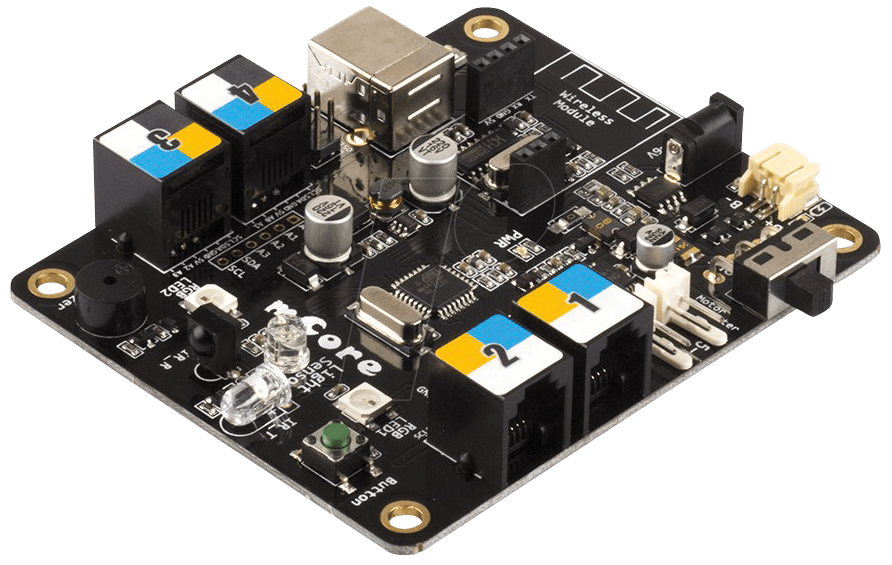
\includegraphics[width=8cm]{mcore.png}\centering
	\label{img:Mcore}
	\caption{Placa mCore}
\end{figure}
\subsection{MBot}\label{subsec:mbot}
Actualmente hay una gran variedad de robots educativos, orientados principalmente a los alumnos más jóvenes. El objetivo de la robótica educativa es ofrecer un entorno amigable y divertido, además de \textit{más realista} que la programación tradicional. Es más fácil para un niño o niña sentirse interesado por algo que tiene una reacción \textit{visible}, en algo que puede tocar y manejar, que en la programación normal que, aunque produce una reacción, es mucho más abstracta. Esto convierte la robótica en la herramienta perfecta para enseñar lenguajes, conceptos básicos de programación como funciones, uso de variables, y avanzar hasta la algoritmia se hace un proceso natural al que los propios alumnos llegan ellos mismos. \\
El principal problema al que nos enfrentamos para enseñar programación a los más jóvenes son los lenguajes de programación. Son poco intuitivos y legibles, sumado a la dificultad de mantener la atención de un alumno o alumna tan joven escribiendo en un ordenador en estos lenguajes. Era necesaria, por tanto, una forma de enseñar estos conceptos de programación comentados anteriormente sin tener que utilizar lenguajes clásicos de programación, al menos para los alumnos más jóvenes. La solución fue la programación por bloques de \textit{pseudocódigo}. El pseudocódigo es un \textit{framework}, una carcasa, que recubre el verdadero lenguaje de programación de la placa del robot, y lo hace legible y entendible. Además, siendo esto una de las grandes ventajas añadidas, la mayoría de los pseudocódigos están en casi todos los idiomas, permitiendo a los alumnos programar en su propio idioma. \\
\par Esto nos lleva al robot Mbot (\cite{makeblock}). Está basado en una placa Arduino Uno, y pensado especialmente para la enseñanza: los diferentes sensores y actuadores (los que vienen en el paquete básico, aunque hay muchos más posibles del mismo fabricante)están pensados para ofrecer prácticas entretenidas y, lo más importante, con diferentes niveles de dificultad, por lo que se puede utilizar con alumnos de diferentes edades y, durante un mismo curso escolar, crear prácticas con las que evolucionar en los conceptos. 
\begin{figure}[H]
	\includegraphics[width=8cm]{Mbot.jpg}\centering
	\label{img:mbot}\caption{Modelo Mbot utilizado}
\end{figure}
Este robot Mbot se programa utilizando un  lenguaje llamado \textit{Scratch} (\ref{subsec:scratch}),  un pseudo código muy gráfico y sencillo pero potente, que ''recubre'' la placa base. Sin embargo, al ser una placa Arduino y por lo tanto, reprogramable, siempre se puede programar en el propio lenguaje Arduino. Esto  se comentará en profundidad más adelante, en el punto \ref{cap:PyBoKids}. \\
Como se puede observar en la imagen, el robot cuenta con dos motores conectados a la placa; contiene además cuatro puertos a los que poder conectar diferentes periféricos con los que trabajar (numerados del uno al cuatro), sin contar con los motores. El modelo mostrado es el básico, sin embargo se pueden cambiar los componentes, añadiendo y/o cambiando la estructura base, y crear ''otro'' robot (por ejemplo, en las figuras siguientes \ref{img:mbot2} ). Aunque en este Trabajo de Fin de Grado solo trabajaremos con la versión básica del Mbot, esta posibilidad de añadirle componentes o cambiarlos es muy interesante para los alumnos, ya que trabajan la mecánica y pueden utilizar más tipos de periféricos.
\begin{figure}[H]
	\includegraphics[width=6cm]{Mbot-pack-piernas.jpg}
	\includegraphics[width=6cm]{Mbot-pack-piernas2.jpg}
	\centering
	\label{img:mbot2}\caption{Posibles cambios en el Mbot}
\end{figure}
\subsubsection{Sensores}\label{ssubsec:sensores}
En robótica un \textit{sensor} es un periférico de entrada que, conectado a una placa base, recoge información del medio (cantidad de ruido, temperatura, distancia frontal, etc) y la envía a la placa, dejándola disponible para toma de decisiones. La cantidad de información que se pueda recibir sólo depende de la cantidad de sensores que se pueda conectar a la vez a la placa (cuatro, en este caso, si solo se trabajara con sensores y ningún actuador). En el robot básico (de la imagen \ref{img:mbot}) los sensores son:
\begin{description}
	\item [Sensor de ultrasonidos] Está colocado en el frente, y recoge información de \textbf{distancia} hasta un objeto, en \textit{cm} (el valor máximo es 400)
	
	\item [Sensor infrarrojo \textit{Sigue Líneas}] Está ubicado de tal forma que lea, del ''suelo'', si el sensor está tapado o no, es decir: está sobre blanco o negro (de fondo, es un sensor binario). Se compone en realidad de dos sensores, izquierdo y derecho, por lo que habrá cuatro posibilidades, cada una codificada con un valor numérico (el valor que devuelve el sensor a la placa Arduino):
	\begin{itemize}
		\item Ningún sensor tapado: 0
		\item Sensor izquierdo tapado y derecho no: 1
		\item Sensor derecho tapado e izquierdo no: 2
		\item Los dos sensores tapados: 3
	\end{itemize}
	 \item [Sensor de Luz] En este caso, está integrado en la placa, por lo que no es necesario utilizar un puerto para él. Nos da un valor de cantidad de luz en el ambiente, pudiéndolo utilizar para saber si hay más o menos luminosidad de la deseada. Por supuesto, para este valor ''deseado'' será necesario obtener un valor inicial de la habitación en la que nos encontremos, para poder establecer ese valor barrera (\textit{threshold})
\end{description}
\begin{figure}[H]
	\begin{center}
		\begin{subfigure}
			[Ultrasonidos: sensor de distancia]{
			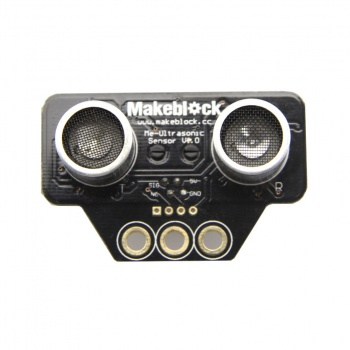
\includegraphics[width=0.45\textwidth]{ultrasonidos.jpg}
			\label{img:ultrasonidos}}
		\end{subfigure}
		\begin{subfigure}
			[Infrarrojos: sensor siguelíneas]{			
			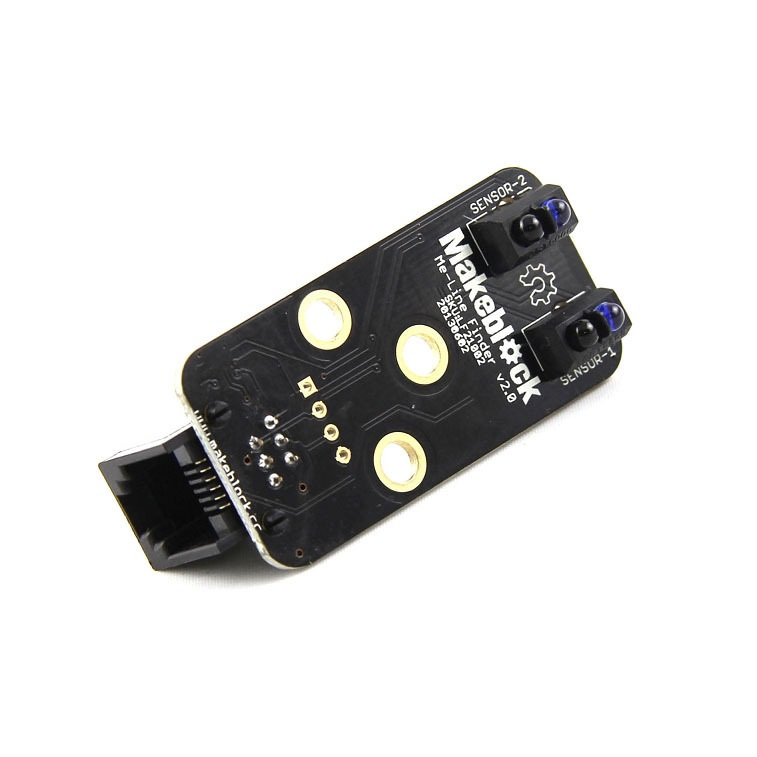
\includegraphics[width=0.45\textwidth]{siguelineas.jpg}
			\label{img:siguelineas}}
		\end{subfigure}
		\begin{subfigure}
			[sensor de luz integrado]{			
			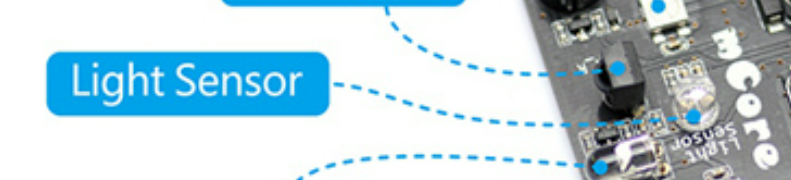
\includegraphics[width=0.45\textwidth]{sensorLuz.png}
			\label{img:sensorluz}}
		\end{subfigure}
	\label{img:sensores}
	\caption{Sensores}
	\end{center}
\end{figure}


\subsubsection{Actuadores}\label{subsec:actuadores}
	La definición de \textit{actuador} es un periférico de salida al que la placa envía datos con los que éste realiza una acción de una forma u otra. Por ejemplo, teniendo una velocidad $v_0$, este valor es enviado a los motores, que se moverán a esa velocidad y no a otra. \\
	Los actuadores, los que no están integrados en la placa directamente, se conectan a la placa a través de los mismos puertos que los sensores. Para poder usarlos, habrá que especificarle a la placa en qué puerto están conectados (igual que con los sensores). En nuestro robot básico, tenemos los siguientes actuadores:
	\begin{description}
		\item [Leds]. Están integrados en la placa, en la parte superior, y compuesto por dos led individuales que poder combinar dependiendo de qué valor codificado se envíe a la placa:
		\begin{itemize}
			\item Los dos led: 0
			\item Sólo led derecho: 1
			\item Sólo led izquierdo: 2
		\end{itemize}
		Los led son RGB (\textit{[red, green, blue]}), y el color de los dos led se codifica con un valor entre 0 y 255 para cada uno de los colores rojo, verde y azul. Así, por ejemplo, el rojo completo sería [0,255,0], el morado sería [255,0,255], el negro [0,0,0] o el blanco [255,255,255]. Estos led están codificados con valores decimales, en vez de hexadecimales como sería una codificación RGB tradicional, para facilitar la programación a los alumnos, que no conocerían el sistema hexadecimal.
		\begin{figure}[H]
			\includegraphics[width=3cm]{RGBled.png}
			\centering
			\label{img:led}
			\caption{Led RGB integrados}
		\end{figure}
		\item [Motores] En el paquete básico tenemos dos motores DC (de corriente continua) conectados a la placa en un conector específico para motores a los que conectar los dos cables, positivo y negativo. Los motores admiten como velocidad de entrada valores enteros entre [-255,255] (valores negativos para retroceder y positivos para avanzar), pudiendo dar valores diferentes a cada uno de ellos (para tener capacidad de hacer girar al robot).
		\begin{figure}[H]
			\begin{center}
				\begin{subfigure}
					[Puerto de conexión de los motores]{
						\includegraphics[width=0.45\textwidth]{puertomotor.png}
						\label{img:puertomotor}}
				\end{subfigure}
				\begin{subfigure}
					[Motor DC]{			
						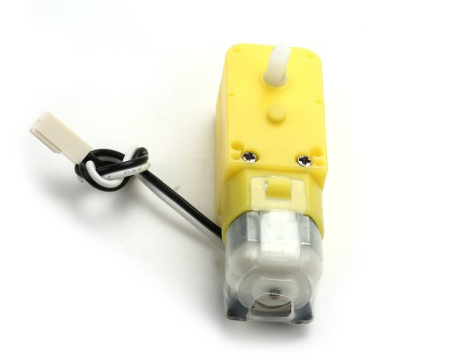
\includegraphics[width=0.33\textwidth]{motorDC2.png}
						\label{img:motor1}}
				\end{subfigure}
				\begin{subfigure}
					[Motor DC: montaje con rueda]{			
						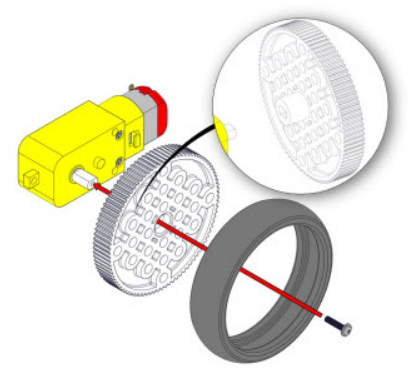
\includegraphics[width=0.33\textwidth]{motorDC.png}
						\label{img:motor2}}
				\end{subfigure}
				\label{img:motores}
				\caption{Motores}
			\end{center}
		\end{figure}
	
	\item [Zumbador] También integrado en la placa, emite notas musicales codificadas en nomenclatura americana. La equivalencia, que los alumnos necesitan conocer, está en la tabla siguiente. Para utilizar diferentes notas más agudas o más graves, se utilizan números a continuación de las letras (\textbf{C0} es más grave que \textbf{C5}). Internamente, el zumbador entiende valores enteros, correspondientes en frecuencia con cada nota (en la tabla, sólo se pone el valor para los valores \textit{1}, a modo de ejemplo):
	\begin{table}[h]
		\centering
		\begin{tabular}{ c | c | c}	
			Europea & Americana & Valor entero \\
			\hline			
			Do & C & 33\\
			RE & D & 37\\
			MI & E & 41\\
			FA & F & 44\\
			SOL & G & 49\\
			LA & A & 55\\
			SI & B & 62\\
		\end{tabular}
	\label{table:notasZumbador}
	\caption{Relación entre notas para el Zumbador del mBot}
	\end{table}

	
	\begin{figure}[H]
		\includegraphics[width=3cm]{buzzer.png}
		\centering
		\label{img:zumbador}
		\caption{Zumbador integrado}
	\end{figure}
\end{description}



\section{Software}\label{sec:software}
En esta sección describiremos el diferente software utilizado y el propósito de éste en el marco de este Trabajo Fin de Grado. 

\subsection{Scratch y mBlock}\label{subsec:scratch}
Como se ha comentado anteriormente, el robot Mbot es programable con Scratch, un lenguaje de \textbf{programación por bloques}. Un \textit{bloque de código} consiste en codificar en un ''paquete'' una sentencia completa de lenguaje (del lenguaje correspondiente, Arduino en este caso). Así, el estudiante que utilice Scratch, será capaz de utilizar una sentencia \textit{if..else} o un bucle \textit{for} de forma muy fácil y entendible, sin necesitar aprenderse todas las reglas de sintaxis del lenguaje real. A continuación, se muestran algunos ejemplos de bloques en Scratch correspondientes a los conceptos de programación más utilizados:
\begin{figure}[H]
	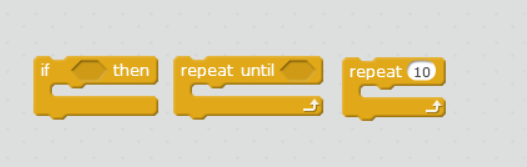
\includegraphics[]{scratch.png}
	\centering
	\label{img:scratch}
	\caption{Algunos ejemplos de bloques en Scratch}
\end{figure}
Como puede observarse, las sentencias que se quieran repetir, o las variables de condición, tienen un lugar muy intuitivo donde colocarse. Además, pueden crearse variables, en las que guardar los valores de los sensores y poder utilizar como entrada de actuadores, o como valores de referencia. \\
Ciertamente, y aunque el lenguaje Scratch puede utilizarse como lenguaje de programación ''tradicional'', utilizando un escenario virtual con un personaje para observar el resultado del programa (sin robot físico), es mucho más completo al añadirle el módulo del robot deseado. Este módulo contiene bloques para recoger valores de los sensores o enviar valores a los actuadores, ya sean \textit{''on board''} (integrados en la placa), o teniendo que especificar el puerto al que están conectados:
\begin{figure}[H]
	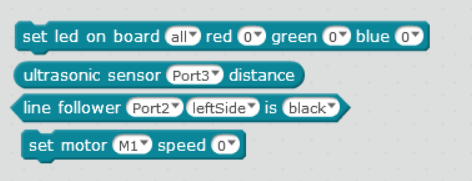
\includegraphics[]{scratch2.png}
	\centering
	\label{img:scratch2}
	\caption{Ejemplos de bloques de Mbot en Scratch}
\end{figure}

Para utilizar Scratch y programar el robot, es necesario instalar un programa, que es el que contiene el compilador y el que permite conectar el robot al PC para enviarle el programa, llamado \textit{mBlock}. El ejecutable se descarga de la página oficial del fabricante, \href{https://www.makeblock.es/blog/descargas/}{Makeblock}, disponible para PC (también existe una versión simplificada para dispositivos móviles).\\
Una vez instalado el software, el proceso para poder empezar a usar el mBot es muy simple:
\begin{enumerate}\label{list:conexionMblock}
	\item Conectar el robot al pc con el cable USB, y conectarlo con el programa (el robot debe estar encendido).
	\begin{figure}[H]
		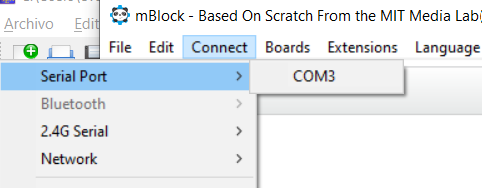
\includegraphics[]{mblock.png}
		\centering
		\label{img:mblock}
		\caption{Conectar el mBot}
	\end{figure}

	\item  Asegurarse de que la placa corresponde con el robot que tenemos
	\begin{figure}[H]
		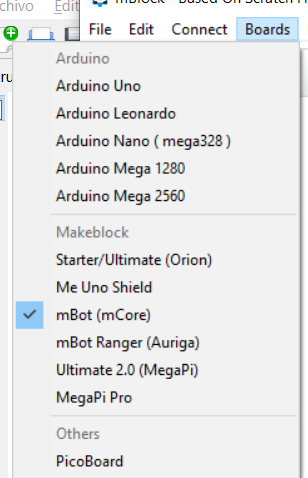
\includegraphics[]{mblock2.png}
		\centering
		\label{img:mblock2}
		\caption{Placa mBot}
	\end{figure}

	\item Actualizar el programa Arduino subido a la placa base, para que funcione con Scratch (en caso de haber utilizado el robot con otro programa)
	\begin{figure}[H]
		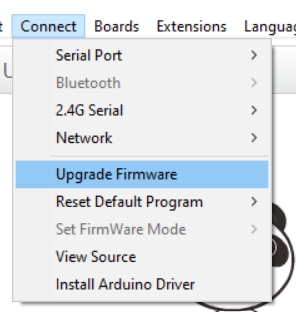
\includegraphics[]{mblock3.png}
		\centering
		\label{img:mblock3}
		\caption{Actualizar firmware de la placa}
	\end{figure}

	\item Una vez programado algo de código, para subirlo al robot: click derecho sobre el código, 'upload to arduino', para compilar el programa, y otra vez a 'upload to arduino' cuando el compilador aparezca en la parte derecha de la pantalla, para subirlo a la placa
	\begin{figure}[H]}
		\centering
		\begin{subfigure}
			[Compilar programa]{
				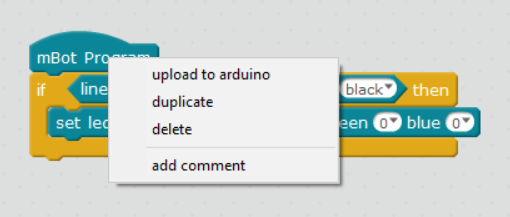
\includegraphics[width=0.45\textwidth]{mblock4.png}
				\label{img:uploadArduino1}}
		\end{subfigure}
		\begin{subfigure}
			[Subir programa a la placa]{
				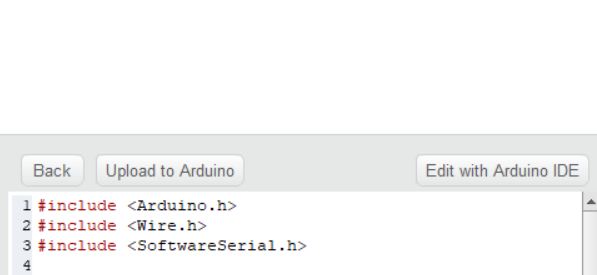
\includegraphics[width=0.5\textwidth]{mblock5.png}
				\label{img:uploadArduino2}}
		\end{subfigure}
	\caption{Subir programa a la placa del mBot}
	\end{figure}

	\item Una vez subido el programa, el robot comenzará a funcionar tal y como lo hayamos programado.
\end{enumerate}
 

\par Este lenguaje, junto a la interfaz gráfica, es una perfecta primera aproximación a la programación y a la robótica, dando más importancia al aprendizaje conceptual que a la sintaxis y al lenguaje. \\
Obviamente, los alumnos necesitarán que se les guíe, principalmente al comienzo del curso, en comprender las necesidades de incluir los diferentes bloques y las ventajas que produce en el código. El objetivo no será explicarles para que usar, por ejemplo, un bloque condicional,  sino proponerles un ejercicio en el que, para llegar a la solución, necesitarán de forma intuitiva programar un condicional, y lleguen naturalmente a la necesidad de ello.
\subsection{Arduino}\label{subsec:arduino}
Como se explicó cuando hablamos de la placa base en la sección \ref{subsec:placaBase}, ésta se programa en \textbf{Arduino}. Este lenguaje de programación está basado en C++, y pensado para interactuar con objetos electrónicos. \\
Teniendo en cuenta el objetivo de este Trabajo Fin de Grado, ofrecer una posibilidad de programar el robot Mbot en Python, es necesario utilizar el lenguaje nativo de la placa base, con el fin de que el robot \textit{entienda} las órdenes programadas en Python. Por lo tanto, para crear este ''framework'', es necesario instalar el entorno Arduino. A continuación se explican las instrucciones para instalar el entorno en Windows, y para configurarlo para el robot.
\begin{enumerate}\label{list:InstalacionArduino}
	\item Descargar e instalar, Arduino IDE, el cual instala el entorno completo de Arduino. Para las versiones 8 y 10 de Windows, está disponible directamente en el Microsoft Store. Para otras versiones de Windows, está disponible en la  \href{https://www.arduino.cc/en/software}{página web oficial}.
	\begin{figure}[h]
		\includegraphics[width=10cm]{store.png}
		\centering
		\label{img:MStore}
		\caption{Arduino IDE en el Microsoft Store}
	\end{figure}
	\item Descargar las librerías de \href{https://codeload.github.com/Makeblock-official/Makeblock-Libraries/zip/master}{Makeblock} o del \href{https://github.com/JdeRobot/PyBoKids/tree/main/PyBoKids%202.0}{repositorio PyBoKids} para añadirlas a Arduino y poder utilizarlas en nuestro entorno.
	\item Incluir el archivo comprimido descargado desde el Arduino IDE:\\ \textit{Programa - Incluir librería - Añadir biblioteca .ZIP - Seleccionar el fichero - Abrir}
	\item Seleccionar la placa básica que se va a conectar al IDE:\\
	\textit{Herramientas - Placa - Seleccionar Arduino Uno}
	\item Especificar el modelo exacto de placa al principio del programa de Arduino; en este caso la placa que estábamos utilizando es la mCore. Así se cargan todos los métodos correspondientes al modelo de placa; debe incluirse en cada programa de Arduino que se escriba.
	\begin{verbatim}	
		#include "MeMCore.h"	
	\end{verbatim}
	\item Igual que con Scratch, primero se debe conectar el robot al software (con el robot enchufado al PC y encendido):\\
	\textit{Herramientas - Puerto - Seleccionar el puerto en el que está el robot} \\
	Los puertos USB en Windows son \textit{COM1, COM2, COM3}, etc.
	\item  Una vez tengamos un programa en Arduino listo para subir a la placa y probar con el robot:\\
	\textit{Programa - Subir } o el botón rápido de ''subir''. \\
	Este proceso primero compilar el programa y, si está correcto, lo sube a la placa. Sin embargo, se puede compilar primero como comprobación \textit{(Programa - Verificar)}.
\end{enumerate}
\subsection{Python}\label{subsec:python}
Por último, utilizaremos \textbf{python} para programar la lógica de los ejercicios. El objetivo es que se programe en python sólo los ejercicios, habiendo paquetizado todo lo relativo al robot en Arduino, y sólo utilizando la conexión con éste para obtener datos de los sensores y enviar datos a los actuadores. La descripción de este proceso y de la lógica de ambos lados (PC y robot) se describirá en profundida en el capítulo \ref{cap:PyBoKids}.
\par La razón de utilizar Python como lenguaje de programación es la misma que la del resto de componentes: la facilidad para los alumnos de acceder a ello. Es uno de los lenguajes con sintaxis más simple (por comparación, Arduino / C++ es muy cerrado y complejo), además de ser las palabras reservadas significantemente entendibles (aunque es cierto que en inglés: \textit{while}, \textit{print}, \textit{read}, etc), así como la declaración de variables es más flexible. Además, y aparte de la cuestión educacional, el módulo \textit{serial} para conexión con periféricos, está con la instalación base, y es mucho más sencillo que en otros lenguajes, haciéndolo perfecto para la electrónica. 
\par La instalación de python en Windows también es muy sencilla:
\begin{enumerate}\label{list:instalacionPython}
	\item Descargar el paquete de la \href{https://www.python.org/downloads/}{web oficia} y ejecutar el instalable descargado.
	También es posible, para Windows 10, obtenerlo desde el Microsoft Store, tal y como se hizo para Arduino.
	\item Una vez descargado, comprobar que se puede ejecutar abriendo una consola -Powershell- y escribiendo \textit{python},	se ejecutará la consola de python, y podremos probar que tenemos python instalado en nuestro entorno (\textit{exit()} para salir). También es útil comprobar que hemos instalado la versión correcta (3.10): \textit{python --version} en una consola de Powershell (no teniendo abierta la consola de python)
	\begin{figure}[h]
		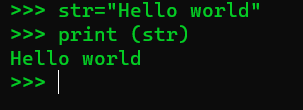
\includegraphics[]{python.png}
		\centering
		\label{img:python}
		\caption{Comprobar python}
	\end{figure}
	\item Para ejecutar un programa escrito en python desde la consola de Windows: 
	\begin{verbatim}
		py HelloWorld.py
	\end{verbatim}
	\item Es probable que la versión de Python, tanto descargada del repositorio oficial como de Microsoft Store no tenga el módulo Serial (necesario para las comunicaciones con el robot) instalado de serie. Tan solo es necesario ejecutar en Powershell la siguiente línea de código:
	\begin{verbatim}
		pip install pyserial
	\end{verbatim}
	\begin{figure}[h]
		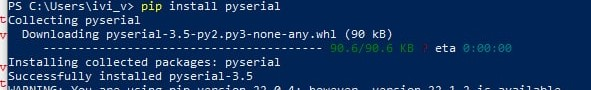
\includegraphics[]{pyserial.jpg}
		\centering
		\label{img:pyserial}
		\caption{Instalar módulo necesario en Python}
	\end{figure}
\end{enumerate}
\newpage
Para escribir código en python, se puede utilizar cualquier editor de texto. El mismo instalador de python instala uno propio, \textit{IDLE shell}, suficientemente simple y preparado particularmente para su sintaxis.

	\chapter{Plataforma PyBoKids 2.0}
\label{cap:PyBoKids}
En este capítulo explicaremos el proceso seguido para desarrollar las bibliotecas Arduino y Python (ver en \cite{arduinolenguaje}, \cite{PythonRef}), explicando el código y las distintas necesidades que han surgido durante el desarrollo. \\
Como se explicó en el Capítulo \ref{cap:infra}, se ha utilizado Arduino  y su IDE nativo para esta programación, y Python 3 y un editor de texto estándar (en este caso, Visual Studio Code, de Microsoft) para la programación en Python. 

\section{Diseño}\label{sec:diseño}
Lo primero en el diseño de la plataforma ha sido el modelo ''PC - Residente''. Partiendo de la premisa dada de programación del robot en Python, era necesaria una forma para que, dado que la placa base funciona en Arduino, la comunicación Serial\footnote{Comunicación secuencial de información a través de un canal, electrónico en este caso} funcionara entre los dos lenguajes. \\

La comunicación con el robot, como se ha comentado en el Capítulo \ref{cap:infra} de Infraestructura, debe establecerse entre el entorno y el robot (con la placa base), cada vez que se encienda éste. Es, por tanto, el primer problema a solventar para ambos entornos. \\ 
El protocolo \textit{Serial} abre una vía de comunicación a través de un canal electrónico, en este caso un cable USB, entre el entorno y el robot, a una velocidad en baudios\footnote{Velocidad, utilizada en electrónica, medida en número de símbolos por segundo}. Este canal para el traspaso de información es necesario para enviar datos a la placa (por ejemplo, los colores a los que encender los LED integrados) o recibir datos de ésta (los valores de lectura de los sensores) y poder utilizarlos en toma de decisiones. \\
Al abrir la comunicación en ambas partes, placa base y PC, cualquiera de ellas es capaz de leer del canal la información que necesite, y de enviar a través de él (para que esto sea así, ambas partes deben haber abierto la comunicación a la misma velocidad). Por tanto, si la placa Arduino envia a través del canal Serial el dato que recoge del sensor de infrarrojos, el lado PC, que estaría leyendo de ese canal, obtendría este dato. \\
En la parte Arduino, al grabar el programa residente completo en la placa, la comunicación se abre a la vez que se enciende el robot, puesto que el programa arranca con él. En la parte PC, de Python, la comunicación se abre cuando ejecutamos el programa que queremos que ejecute el robot. El flujo, entonces, podría dibujarse como el diagrama que aparece a continuación.
\begin{figure}[h]
	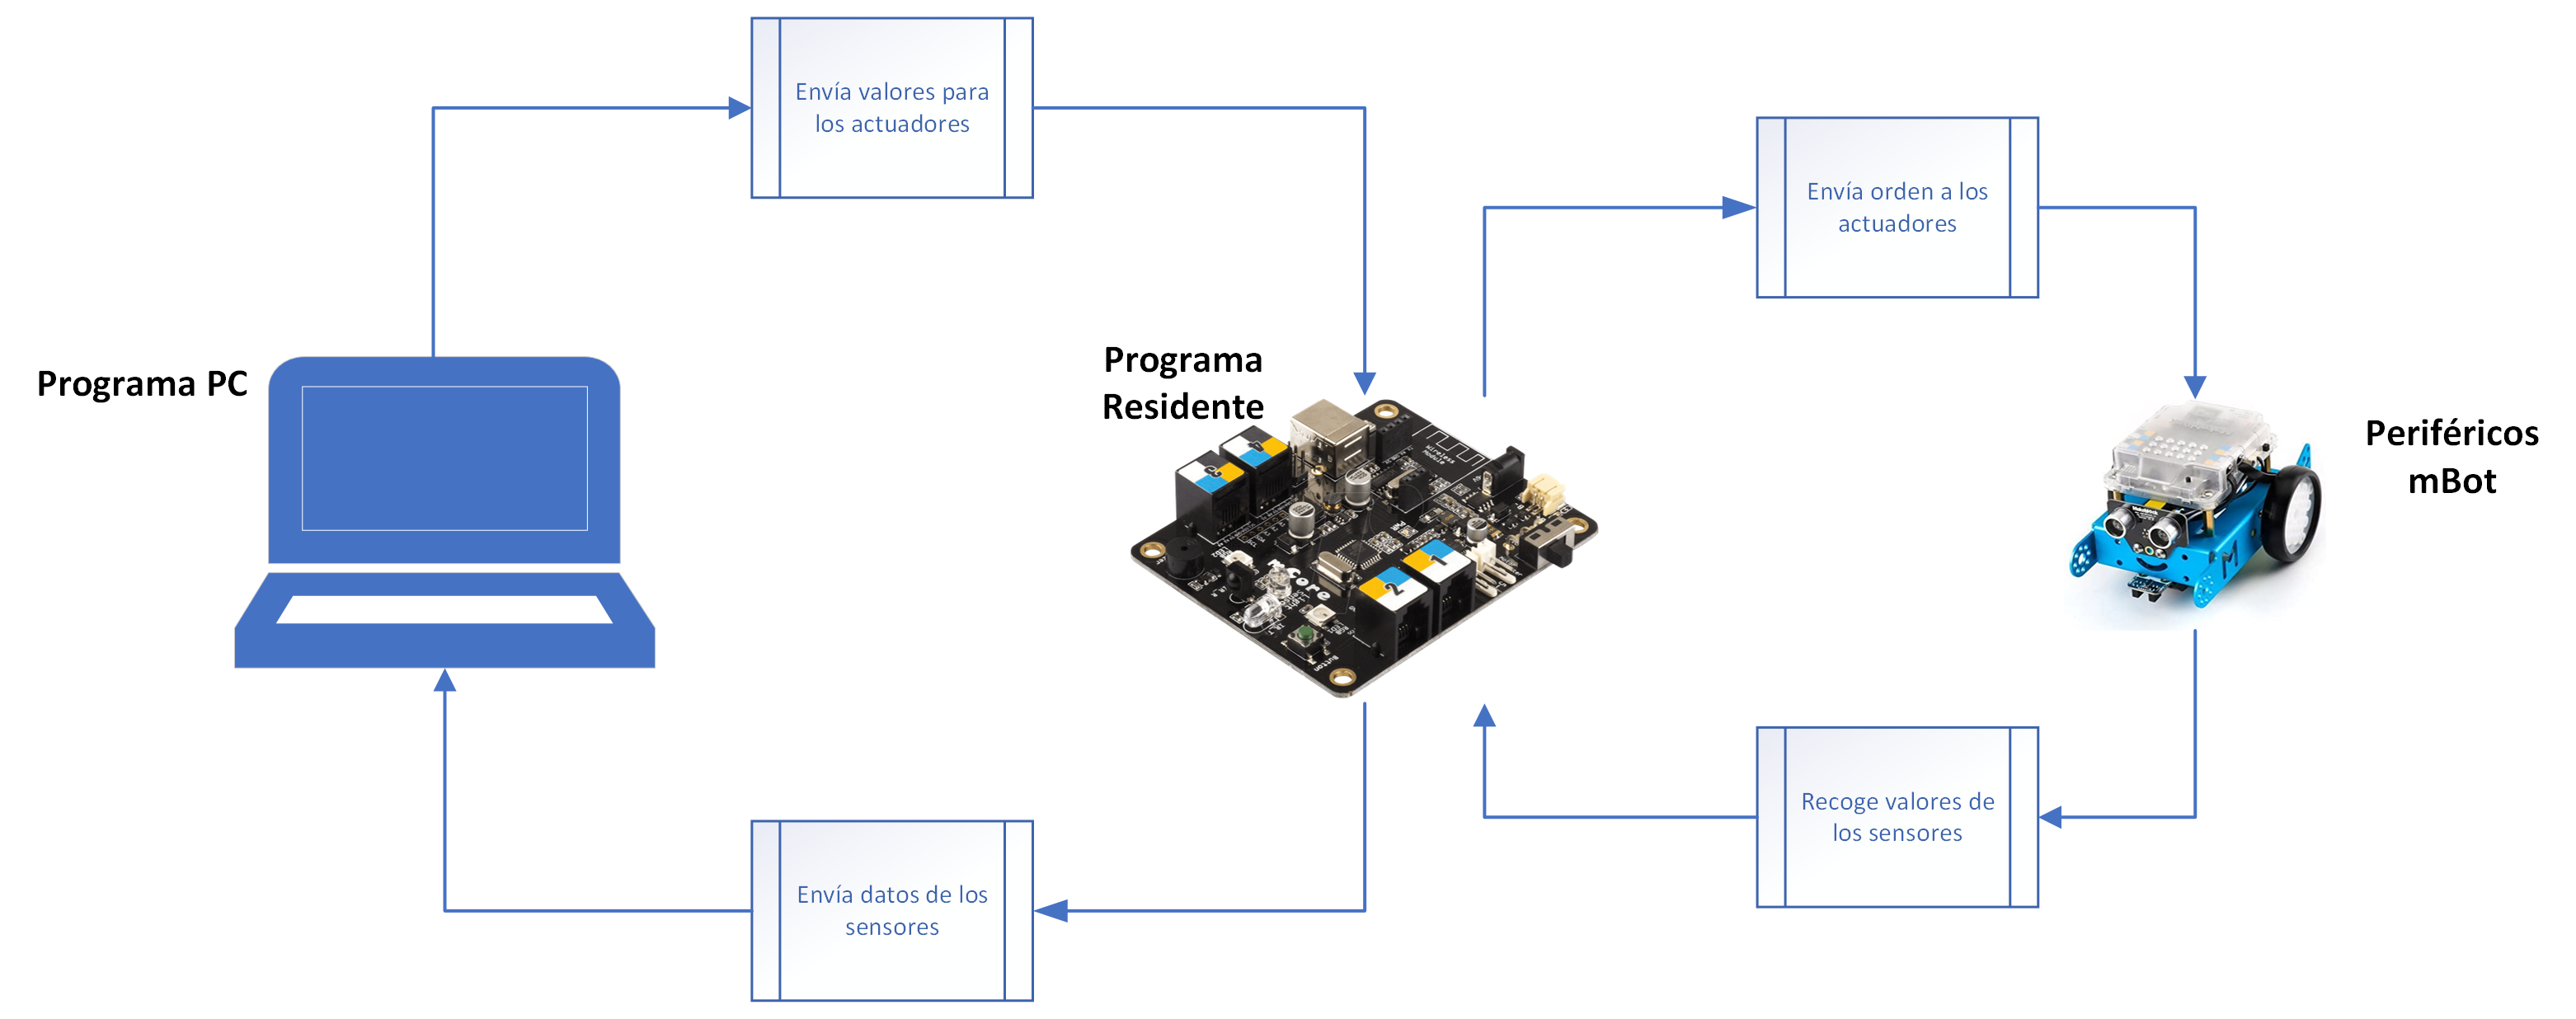
\includegraphics[scale=0.3]{flujo1.png}
	\centering
	\label{img:FlujoComunicaciones}
	\caption{Diagrama de comunicaciones entre PC y Residente}
\end{figure}

\begin{figure}[h]
	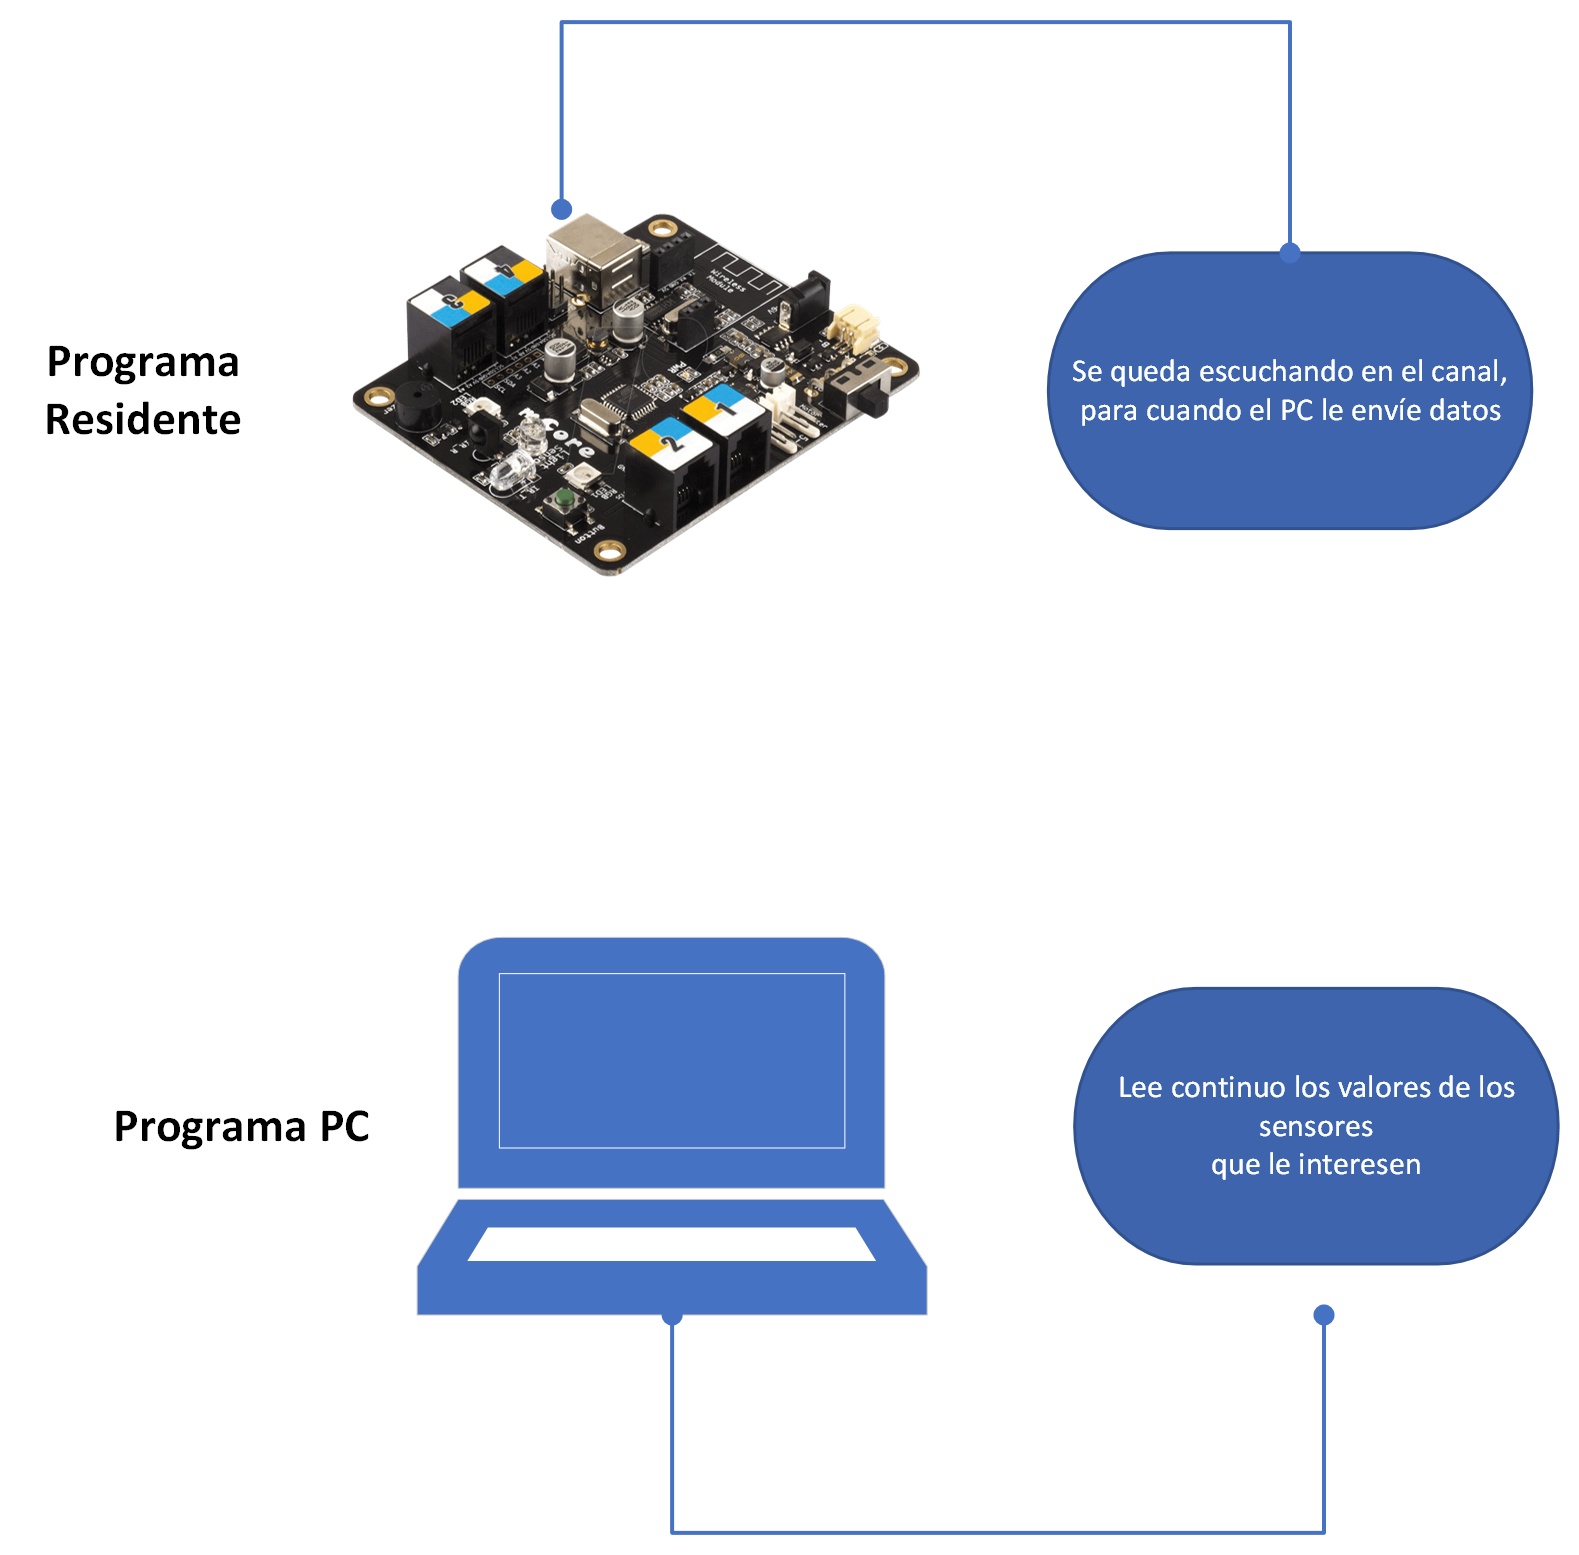
\includegraphics[scale=0.3]{flujo2.png}
	\centering
	\label{img:FlujoComunicaciones2}
	\caption{PC y Residente}
\end{figure}

Como podemos observar, ocurren varias cosas de forma paralela:
\begin{itemize}
	\item El programa residente está recogiendo los valores de los sensores, conectados a su puerto correspondiente, y los envía por el canal.
	\item El programa PC recoge los valores del sensor que le interese (dependerá del programa que queramos uno u otro).
	\item En función del valor del sensor (con respecto a un valor umbral o \textit{threshold}), el programa PC envía por el canal unos valores concretos para un actuador concreto. Lee otra vez el valor -nuevo- del sensor, por si tuviera que cambiar de decisión.
	\item El programa residente lee del canal si tiene mensajes para un actuador y, en caso afirmativo, recoge los valores y los envía al actuador correcto.
\end{itemize}

\section{Protocolo de mensajes}\label{sec:protocolomensajes}
Para que la comunicación entre el programa PC y Residente sea posible es necesario un protocolo de mensajes; es necesario asegurarse que ambas partes recojan la información correcta y sepan qué deben hacer con ella. Poniendo un ejemplo: el Programa Residente debe estar preparado para recibir datos que enviar a los actuadores. Sin embargo, cada actuador requiere datos de entrada diferentes, por tanto, debe estar preparado también para saber para qué actuador le están enviando los datos. Igualmente, el Programa PC debe estar preparado para enviar la información de forma que sea inequívoca. \\
El mismo caso se da para los sensores. El Residente tiene que enviar el dato de forma que el PC pueda saber que el dato que lee es el que necesita (no vale para lo mismo si lee el sensor de luz que el del Sigue Líneas) \\

Este sistema de codificación de los mensajes, funciona de la siguiente forma:
\begin{itemize}
	\item Sensores
	\begin{itemize}			
		\item Dado que la forma más simple, y efectiva debido a ello, de enviar datos es un string, será así como se enviará la información. Para ello, cuando se lea el dato del sensor, habrá que convertir el valor entero en un String. 
		\item A cada sensor se le asignará un número, único (un identificador), que le representará sólo a él. Así, al sensor de ultrasonidos le corresponderá un 0, al Sigue Líneas un 1, etc. 
		\item El Programa Residente, enviará la información en un único mensaje, como String, concatenando el identificador de sensor con el valor de este sensor recogido del robot, separando los dos valores con punto y coma (para diferenciarlo de una posible coma decimal).
		\item El Programa PC, cuando está leyendo, separará el mensaje por ';' y ,dependiendo del primer \textit{substring}, devolverá al programa principal el tipo de sensor en texto, para que sea amigable para un alumno. 
	\end{itemize}
	\begin{figure}[h]
		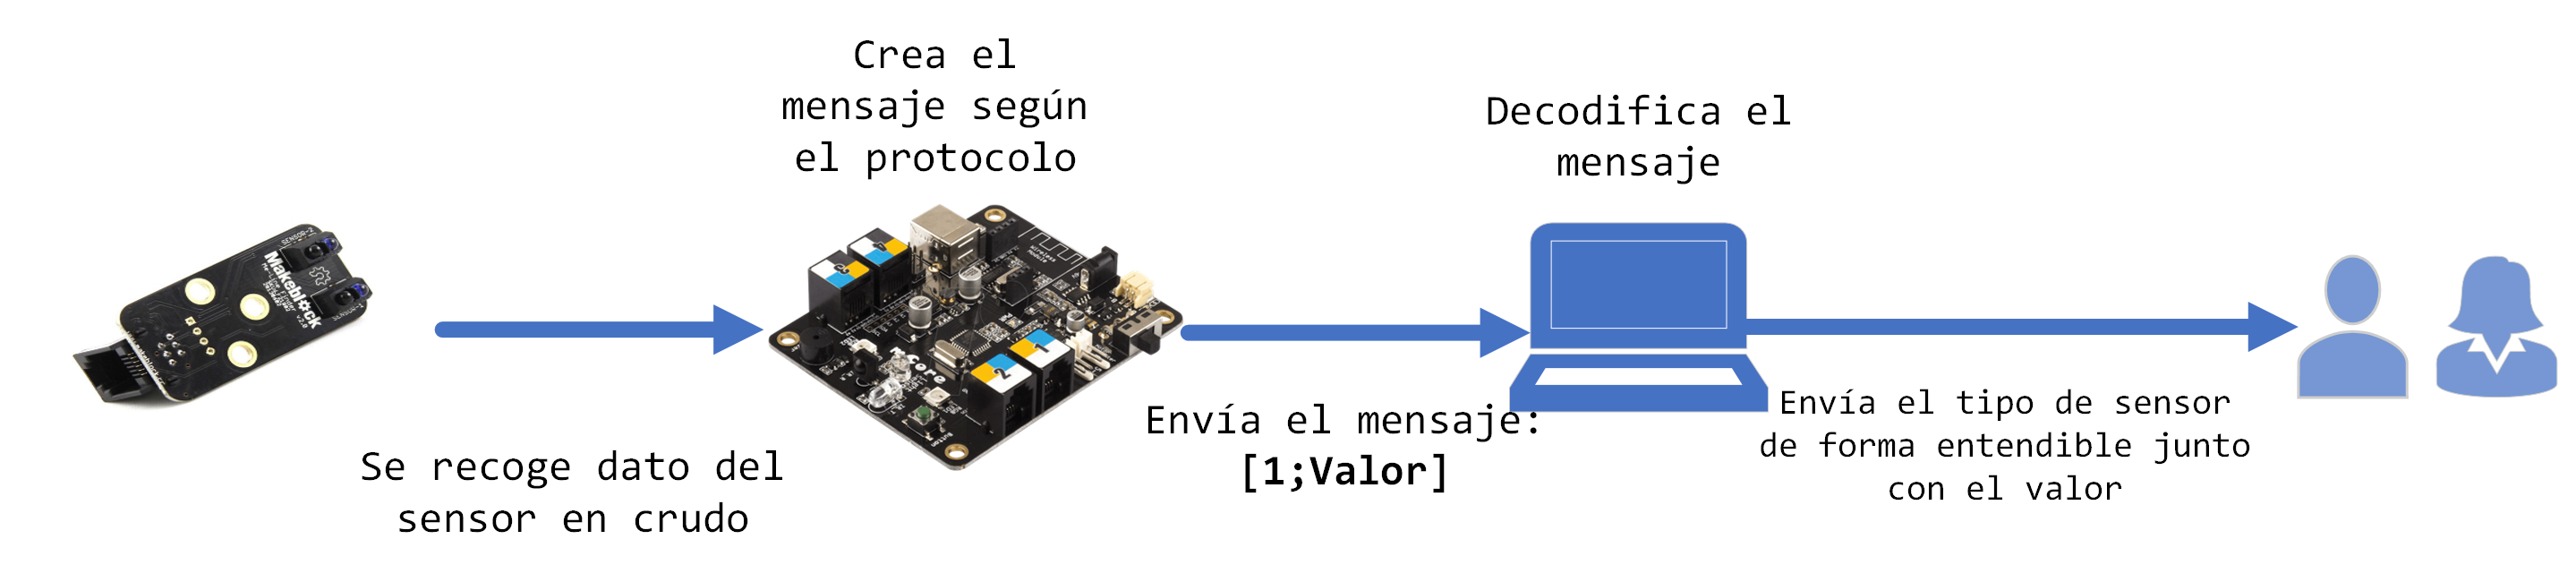
\includegraphics[scale=0.3]{mensajeSensor.png}
		\centering
		\label{img:mensajeSensor}
		\caption{Flujo de mensajes para un sensor}
	\end{figure}
	\item Actuadores
	\begin{itemize}
		\item De forma análoga, a cada actuador se le asignará un identificador numérico.
		\item El Programa PC concatenará, en un mismo mensaje, el identificador del actuador, y los datos necesarios para ese actuador (en caso de los LED, por ejemplo, el valor qué leds encender y los tres valores RGB). Igualmente, todos estos valores irán separados entre ';'. Estos valores serán decididos por el programa principal (por el programador/a).
		\item Al leer del canal, el Residente separará el primer valor por el ';' y dependiendo de qué identificador sea, leerá una cantidad de valores u otra, y enviará esos valores a un actuador u otro (convirtiéndolo primero a valor numérico).
	\end{itemize}
\begin{figure}[h]
	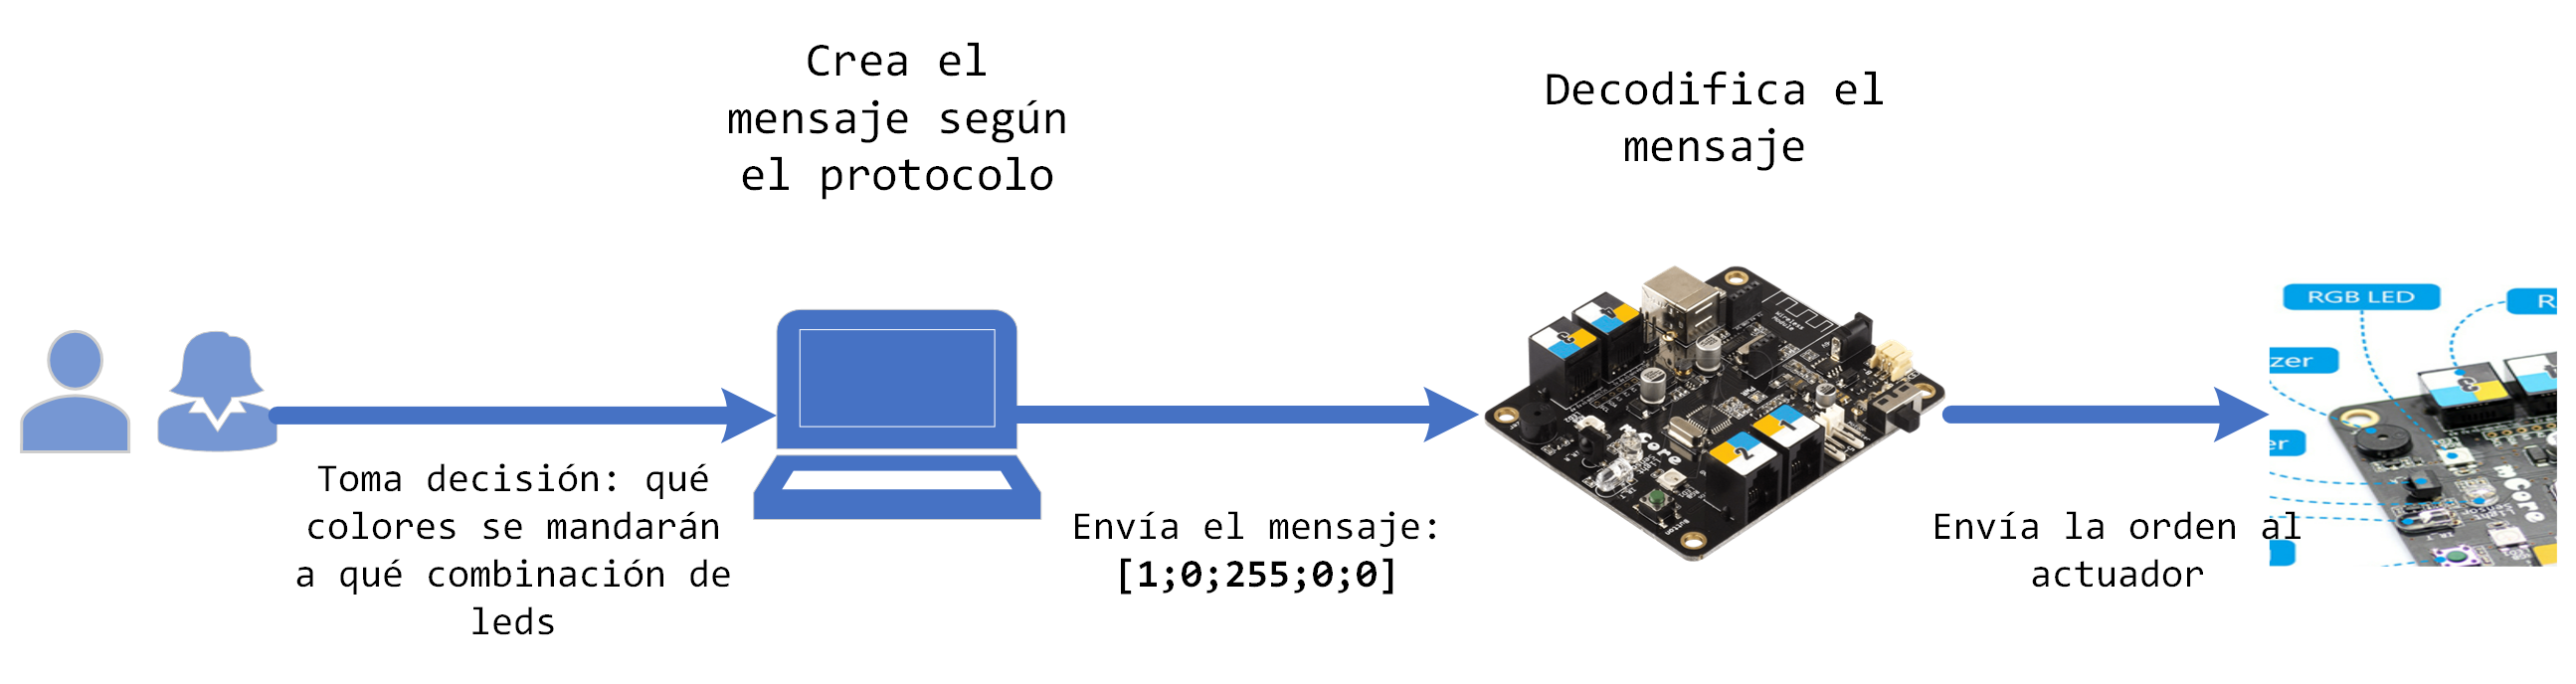
\includegraphics[scale=0.3]{mensajeActuador.png}
	\centering
	\label{img:mensajeActuador}
	\caption{Flujo de mensajes para un sensor}
\end{figure}
\end{itemize}


Con este protocolo de mensajes la funcionalidad de la plataforma PyBoKids 2.0 es fácilmente ampliable a más sensores o actuadores, puesto que los identificadores son números enteros. \\

A continuación, detallaremos la forma técnica en la que se han en la que se ha desarrollado el diseño en ambas partes, Residente y PC, explicando el acceso a los periféricos, la construcción de las bibliotecas y el manejo de este protocolo de mensajes. 
\section{Programa residente en robot}\label{sec:residente}
La biblioteca residente en Arduino se ha realizado de forma progresiva, encontrando diferentes requerimientos y necesidades a lo largo del proceso. 
\subsection{Comunicación serial}\label{subsec:SerialArduino}
En Arduino, para utilizar el protocolo Serial no es necesario cargar ningún módulo añadido, al ser un lenguaje pensado para las comunicaciones electrónicas. La inicialización de la comunicación Serial debe hacerse en la función \textit{setup} de Arduino, donde se coloca el código que debe ejecutarse sólo una vez, al comienzo de la ejecución del programa, con la velocidad en baudios deseada como parámetro.
\begin{lstlisting}[language=C,caption={Inicialización del protocolo Serial},captionpos=b]
void setup() {
  // put your setup code here, to run once:
  Serial.begin(9600);
}
\end{lstlisting}
Durante el resto del código, cada vez que se quiera escribir o leer del canal, deberá llamarse al 'Serial' que hemos iniciado. Es importante comentar que, antes de llamar a una función que lea del canal, debemos asegurarnos que hay datos que poder leer, o el programa generará un error. Por ejemplo:
\begin{lstlisting}[language=C,caption={eco en Arduino: lee del canal Serial y lo escribe},captionpos=b]
char mensaje;
void loop() {
  if (Serial.available()>0)	{
   mensaje = Serial.read();   
   Serial.println(mensaje);
  }
}
\end{lstlisting}
A la hora de leer del canal Serial (en este caso en Arduino, pero igual con cualquier herramienta) hay que tener en cuenta la cantidad de bytes que se leen cada vez. En este caso, estábamos considerando a modo de test, un sólo carácter (inicializando la variable como \textit{char})\footnote{Variable que almacena un valor de carácter, que ocupa un sólo byte de memoria, y que debe escribirse entre comillas simples:\textit{ char mensaje = 'a';}}, por lo que leemos del canal un solo byte (método \textit{read()}). Sin embargo, si quisiéramos leer un \textit{String}\footnote{Array de caracteres, escrito entre comillas dobles, y que termina en valor nulo ('0' en código ASCII): \textit{String mensaje =  "Hello String";}}, como va a ser necesario para leer los mensajes que envíe el programa PC, tendríamos que inicializar la variable como \textit{String} y leer del canal un String entero, esto es, hasta leer el valor nulo en el que éste termina.
\begin{lstlisting}[language=C,caption={eco en Arduino con un Strin},captionpos=b]
String mensaje;
void loop() {
  if (Serial.available()>0) {
   mensaje = Serial.readString();     
   Serial.println(mensaje);
  }
}
\end{lstlisting}

Dado que primero estamos considerando solamente el entorno Arduino, para poder ver el resultado de esta comunicación, usaremos el Monitor Serie del propio IDE de Arduino, que permite escribir por el canal (lo que luego leamos con \textit{serial.readString()}), y muestra lo que Arduino escribe (\textit{Serial.println()}). El código anterior produciría la siguiente ejecución:
\begin{figure}[h]
\centering	
\begin{subfigure}
	[Escribir el String que Arduino lee del canal]{
		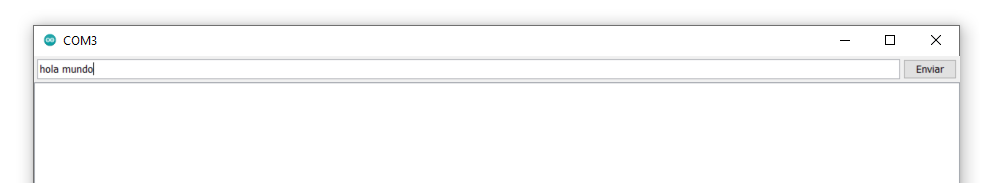
\includegraphics[width=\textwidth]{MonitorEnviar.png}
		\label{img:ComunicacionArduinoEnviar}}
\end{subfigure}
\begin{subfigure}
	[Muestra el String que Arduino ha escrito en el canal]{
		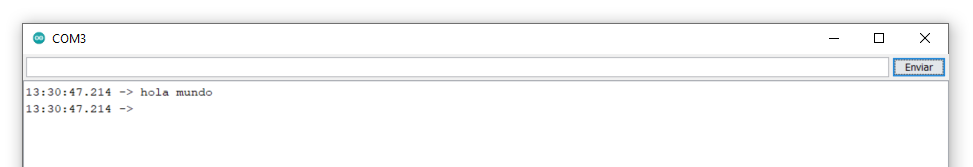
\includegraphics[width=\textwidth]{MonitorRespuesta.png}
		\label{img:ComunicacionArduinoLeer}}
\end{subfigure}
\label{img:ComunicacionArduinoMonitorSerie}
\caption{Visualización del eco de Arduino en el Monitor Serie de Arduino IDE}
\end{figure}

\subsection{Uso de sensores y actuadores}\label{subsec:sensoresyactuadoresArduino}
Una vez comprobadas las comunicaciones, continuamos con los actuadores y sensores del robot. Como se ha explicado en el apartado \ref{subsec:arduino} de Arduino, es necesario cargar los módulos correspondientes a la placa mCore. Una vez incluido el paquete, podremos utilizar los métodos de inicialización, lectura de sensores, envío de órdenes a los actuadores, etc. Este módulo contiene toda la información que necesitan los diferentes componentes (tipos de valores de entrada o de retorno, diferentes métodos, etc), incluidos ejemplos en los que poder apoyarnos. A continuación describiremos como se utilizan los diferentes actuadores y sensores en Arduino, siendo este paso necesario para crear la biblioteca ''Residente''.\\
\begin{itemize}
\item Actuadores: Como cualquier variable, los actuadores requieren de una inicialización; esta inicialización de variables corresponden al principio del programa, para poder utilizar la variable en las funciones principales. Luego, depende de qué actuador sea, requerirá de un tipo u otro de valor de entrada:
\begin{description}
	\item [Motores] Los motores de la placa mCore deben inicializarse cada uno por separado; al darles nombres diferentes podremos enviar la orden al motor correcto (por ejemplo, para girar el robot, no debe enviarse la misma orden al motor derecho que al izquierdo, sino invertir el sentido de uno de ellos, dependiendo de en qué dirección se quiera girar). 
	\begin{lstlisting}[language=C,caption={Inicializar motores Mbot},captionpos=b]	
		MeDCMotor motorIzdo(M1);
		MeDCMotor motorDcho(M2);	
	\end{lstlisting}
	El valor de entrada para la velocidad es un valor entero (tipo \textit{int}), entre [-255,255], siendo los valores negativos para una velocidad de retroceso. En este caso, para que los motores se paren, no se les enviaría un valor de 0 sino que tiene un método propio.	
	\begin{lstlisting}[language=C,caption={Uso de motores Mbot},captionpos=b]		
	motorIzdo.run(100);
	motorDcho.run(100);
	delay (100);
	motorIzdo.stop();
	motorDcho.stop();	
	\end{lstlisting}

	\item [Leds integrados]  En este caso, la inicialización del led requiere el puerto (integrado de la placa) y un slot (de número de leds). Por tanto:
	\begin{lstlisting}[language=C,caption={Inicializar leds},captionpos=b]	
	const int PORT = 7;
	const int SLOT = 2;
	MeRGBLed led(PORT, SLOT);	
	\end{lstlisting}
	Los valores necesarios para los leds se han descrito en la sección de Actuadores \ref{subsec:actuadores}; Arduino requiere primero enviar la configuración de colores, y después mostrar esa configuración. En este caso, para apagarlos, sí se envía un valor de 0 para los tres valores RGB.
	\begin{lstlisting}[language=C,caption={Uso de los leds},captionpos=b]	
	led.setColor(ledsInt,redInt,greenInt,blueInt);
	led.show();	
	\end{lstlisting}

	\item [Zumbador] Como sólo hay un zumbador en la placa, y está integrado en ella, no es necesario ningún puerto. Para que emita la nota deseada, es necesario un valor entero para la frecuencia y otro para la duración (en milisegundos):
	\begin{lstlisting}[language=C,caption={Uso del zumbador},captionpos=b]	
	MeBuzzer buzzer;
	void loop() {
	 buzzer.tone(87,3000);
	 delay(100);
	 // stop the tone playing:
	 buzzer.noTone();
	}
	\end{lstlisting}
\end{description}
\item Sensores: Todos los sensores en Arduino tienen un método de lectura, además del de inicialización. Si queremos almacenar el valor recogido en una variable, Arduino requiere que ésta sea declarada también.
\begin{description}
	\item [Sensor de ultrasonidos] Al no ser un sensor integrado a la placa, es necesario que se especifique en qué puerto se ha conectado. Éste devuelve la distancia, en centímetros (como valor entero), a la que se encuentra un obstáculo.
	\begin{lstlisting}[language=C,caption={Sensor de distancia},captionpos=b]	
	MeUltrasonicSensor ultraSensor(PORT_3);
	void loop() {
	 int DistanceValue = ultraSensor.distanceCm();
	 Serial.println(DistanceValue);
	}
	\end{lstlisting}
	\item [Sensor de luz] El puerto especificado en la llamada al método, aunque integrado en la placa, especifica el pin interno al que está conectado. Devuelve un valor entero, de cantidad de luz. En este caso, para poder utilizar un valor de \textit{threshold} necesitaremos saber qué valor de luminosidad aproximada tiene la habitación (no tiene por qué ser siempre la misma)
	\begin{lstlisting}[language=C,caption={Sensor de luz},captionpos=b]	
	MeLightSensor lightSensor(PORT_6);
	void loop() {
	 int LigthValue = lightSensor.read();
	 Serial.println(LigthValue);
	}
	\end{lstlisting}
	\item [Sensor infrarrojo] Requiere también especificar a qué puerto se le ha conectado, devolviendo de la llamada de lectura un valor entero correspondiente a qué combinación de sensores sigue líneas están tapados o no (explicados en la sección de Actuadores (\ref{subsec:actuadores}))
	\begin{lstlisting}[language=C,caption={Sensor siguelíneas},captionpos=b]	
	MeLineFollower SigueLineas(PORT_1); 
	void loop() {
	 int LineFollowerValue = SigueLineas.readSensors();
	 Serial.println(LineFollowerValue);
	}
	\end{lstlisting}
\end{description}
\end{itemize}

\subsection{Protocolo de mensajes}\label{subsec:mensajesArduino}

Por último, explicaremos cómo se ha desarrollado en el lado Arduino el protocolo de mensajes cuyo diseño está detallado en  \ref{subsubsec:protocolomensajes}. \\
Como se ha comentado, cada sensor y cada actuador tienen un identificador asignado.
\begin{table}[h]
	\centering
	\begin{tabular}{ c | c }
		Periférico & Identificador \\
		\hline			
		Sensor de Distancia &  0\\
		Sensor Sigue Líneas & 1 \\
		Sensor de Luz & 2\\
		\hline
		Leds integrados & 0\\
		Motores & 1\\
		Zumbador & 2 \\

	\end{tabular}
\caption{Relación de periféricos del mBot con su identificador}
\label{table:identificadoresperifericos}
\end{table}
No supone ningún peligro de discrepancia que entre sensores y actuadores tengan identificadores repetidos, ya que los mensajes que lo contienen no van en la misma dirección: los mensajes de los sensores son enviados por el programa Residente y leídos por el programa PC, y los mensajes de los actuadores, del revés.\\

Para utilizar estos mensajes de forma real, necesitaremos en nuestra biblioteca funciones para leer los correspondientes a los sensores, y  componer los de actuadores. \\
Para componer un mensaje para un sensor, las consideraciones a tener en cuenta son: 
\begin{itemize}
	\item Debemos enviar un String, por lo que deberemos convertir a String los valores numéricos.
	\item Los identificadores no pueden cambiarse, por lo que los dejaremos embebidos en el código.
	\item El separador será por punto y coma, para evitar errores en la lectura. Si fuera una coma, podría confundirse con un posible valor numérico decimal del sensor.
\end{itemize} 
\begin{lstlisting}[language=C,caption={Envío de mensajes para los sensores},captionpos=b]
void Send_DistanceMessage () {
	int DistanceValue = ultraSensor.distanceCm();
	String DistanceValueString = String(DistanceValue);
	String DistanceMessage = "0;" + DistanceValueString; 
	Serial.println(DistanceMessage);
}

void Send_LineFollowerMessage () {
	int LineFollowerValue = SigueLineas.readSensors();
	String LineFollowerString = String(LineFollowerValue);
	String LineFollowerMessage = "1;" + LineFollowerString; 
	Serial.println(LineFollowerMessage);
}

void Send_LigthSensorMessage () {
	int LigthValue = lightSensor.read();
	String LigthString = String(LigthValue);
	String LigthMessage = "2;" + LigthString; 
	Serial.println(LigthMessage);
}
\end{lstlisting}

En el caso de los actuadores, dado que son el mensaje ''que llega'' ya formado, para leer debemos:
\begin{itemize}
	\item El mensaje que llega es un String.
	\item Debemos separar ese String por el separador, punto y coma, y almacenar los valores en variables temporales. 
	\item El primer valor que se extraiga, corresponde al tipo de actuador, y dependerá de éste qué lectura del resto del mensaje tenga que hacerse. 
	\item Los valores que deben enviarse como parámetros a los actuadores deberán convertirse en valor numérico, pues es así como lo espera el actuador. 
\end{itemize} 
\begin{lstlisting}[language=C,caption={Decisión sobre los actuadores con el primer valor del mensaje},captionpos=b]
int indexActuator = mensaje.indexOf(';');
String Actuator = mensaje.substring(0,indexActuator);
String mensajeActuador = mensaje.substring(indexActuator+1);
if (Actuator == "0") {
	read_LedsMessage(mensajeActuador);
} else if (Actuator == "1") {
	read_MotorsMessage(mensajeActuador);
} else if (Actuator == "2") {
	read_BuzzerMessage(mensajeActuador);
}
\end{lstlisting}
\begin{lstlisting}[language=C,caption={Lectura de mensajes de los actuadores},captionpos=b]
void read_LedsMessage (String mensaje) {
	int IndexLeds = mensaje.indexOf(';');
	String leds = mensaje.substring(0, IndexLeds);
	int IndexRed = mensaje.indexOf(';', IndexLeds+1); 
	String red = mensaje.substring(IndexLeds+1, IndexRed+1);
	int IndexGreen = mensaje.indexOf(';', IndexRed+1);
	String green = mensaje.substring(IndexRed+1, IndexGreen+1);
	String blue = mensaje.substring(IndexGreen+1,-1); 
	int ledsInt = leds.toInt();
	int redInt = red.toInt();
	int greenInt = green.toInt();
	int blueInt = blue.toInt();
	led.setColor(ledsInt, redInt, greenInt, blueInt);
	led.show();
}	
void read_MotorsMessage (String mensaje) {
	int IndexIzdo = mensaje.indexOf(';');
	String izdo = mensaje.substring(0, IndexIzdo);
	String dcho = mensaje.substring(IndexIzdo+1,-1);	
	int izdoInt = izdo.toInt();
	int dchoInt = dcho.toInt();
	motorIzdo.run(izdoInt);
	motorDcho.run(dchoInt);
}
void read_BuzzerMessage (String mensaje) {
	int IndexNote = mensaje.indexOf(';');
	String note = mensaje.substring(0, IndexNote);  
	String duration = mensaje.substring(IndexNote+1,-1);
	int NoteInt = note.toInt() ;
	int DurationInt = duration.toInt();	
	int durationValue = 1000 * DurationInt;  
	int pauseBetweenNotes = durationValue * 1.30;
	buzzer.tone(NoteInt,durationValue);
	delay(pauseBetweenNotes);
	buzzer.noTone();
}	
\end{lstlisting}

\par Como apunte añadido, y dado que la placa Arduino no se ''apaga'' dejando a neutro todos los valores electrónicos (si apagamos el robot teniendo los led encendidos, cuando se vuelva a encender, lo hará con ellos encendidos), hacía falta una forma de poder apagar todo. En esta biblioteca Residente tendremos las funciones correspondientes para dejar apagados cada actuador con sus valores correspondientes:

\begin{lstlisting}[language=C,caption={Apagado de los actuadores},captionpos=b]
void Stop_Motors () {
	motorIzdo.stop();
	motorDcho.stop();
}

void Stop_Leds () {
	led.setColor(0, 0, 0, 0);
	led.show();
}

void Stop_Buzzer () {
	buzzer.noTone();
}	
\end{lstlisting}

Esta funcionalidad de ''apagado'' se pedirá con un mensaje desde el programa PC, que controlaremos en Arduino al principio de lectura del mensaje:

\begin{lstlisting}[language=C,caption={Apagado de los actuadores},captionpos=b]
String mensaje = Serial.readString();
if (mensaje.equalsIgnoreCase("quit")) {
	Stop_Motors();
	Stop_Leds();
	Stop_Buzzer();
	exit(0);
}
\end{lstlisting}

Una vez conocido el funcionamiento de los componentes del mBot, hemos podido abstraer este conocimiento y desarrollar las funciones que compondrán esta biblioteca Arduino. Estas funciones crearán la estructura del programa residente de forma que funcione independientemente de qué datos se le envíen desde el programa PC.

\section{Programa PC}\label{sec:pc}
La finalidad del Programa PC es tener una biblioteca de funciones que contengan la lógica de conexión, lectura, escritura, etc, y que la escondan a los alumnos, teniendo ellos que preocuparse solamente de llamar a una función con un nombre amigable. A continuación describiremos los puntos importantes que se han necesitado en la preparación de esta biblioteca.
\subsection{Comunicación Serial}\label{subssec:serialPython}

En este caso, es necesario incluir el módulo Serial al principio del programa de Python. Para iniciar una comunicación Serial, al igual que con Arduino, es necesaria la velocidad en baudios a la que conectarse (como dijimos, debe ser la misma a la que se ha abierto la comunicación en la parte de Arduino); además es necesario el puerto al que está conectado el robot (de forma parecida a la que se especificaba en el Arduino IDE) y un tiempo de \textit{timeout} para el que, si no se ha establecido la comunicación, se eleva una excepción (que se deberá recoger con un bloque de \textit{try..catch}). 
\begin{lstlisting}[language=python,caption={Función de la biblioteca Python para abrir el puerto serie},captionpos=b]	
def open_PortSerial (port):
	try:
		serialAux = serial.Serial(115200, port, timeout=1)
		serialAux.setDTR(False)
		sleep(1)
		serialAux.flushInput()
		serialAux.setDTR(True)
		sleep (1)
		return serialAux
	except serial.SerialException:
		sys.stderr.write("Error al abrir puerto (%s)\n")
		sys.exit(1)
\end{lstlisting}

La velocidad a la que funcione la comunicación Serial se ha establecido finalmente en 115200 baudios ya que, de forma experimental, al añadir los sensores fue necesario subir el valor para mantener la comunicación de forma útil. Este valor se establece como constante, para asegurarnos que es el mismo valor en las dos partes PC y Residente. 

\paragraph {Leer del canal} 
Para leer del canal, deberemos tener en cuenta igualmente la cantidad de información que queramos leer. En general, como estaremos leyendo mensajes tipo String, Python contiene (como Arduino) la función de lectura de una línea completa (hasta fin de línea). 
\begin{lstlisting}[language=python]
serial.readline() #leer hasta EOL		
\end{lstlisting}
Sin embargo, es posible leer un solo byte (como en el caso de leer un solo carácter), o una cantidad de bytes especificada.

Dado que el String leído con el valor de un sensor, lo ha enviado Arduino y ha atravesado el canal, es necesario decodificarlo para obtener un String sin los caracteres de retorno de carro, end of line, etc. Si no, no podríamos utilizar como número ese valor, ya que al intentar convertirlo desde String, no debe tener ningún otro carácter.
\begin{lstlisting}[language=python]	
Data = serial.readline()
decoded = Data.decode()
sensorValue = float(decoded)
\end{lstlisting}
	
	
\paragraph {Escribir en el canal} Al igual que para leer, para escribir en el canal y asegurarnos que en al programa residente le llegan datos que sea capaz de interpretar, el envío de datos (texto) debe hacerse forzando la codificación en UTF-8.
\begin{lstlisting}[language=python]
Data = "Hello World"
serial.write(bytes(Data, 'utf-8'))
\end{lstlisting}

Estas decisiones de codificaciones, tanto para escribir como para leer del canal, son el resultado de pruebas entre uno y otro lado (Arduino - Python), con varios tipos de datos y de formas de leer del canal (bytes, Strings, etc), con la finalidad de asegurar que ambos lados pueden establecer una comunicación con éxito y que las opciones necesarias están recogidas.

\subsection{Protocolo de mensajes}\label{subsec:mensajesPython}
En el caso de la biblioteca Python, no debemos preocuparnos de los sensores y actuadores como Hardware, ya que el programa PC no lee directamente de ellos, sino que se comunica con la placa base (con el programa Residente). Por tanto, deberemos establecer la lectura y envío de los mensajes, en este caso del revés que en el lado Residente: la lectura y decodificación serán para los sensores, y el envío para los actuadores. La biblioteca contendrá toda esta funcionalidad ''escondida'' para que los alumnos utilicen simplemente funciones con nombres autoexplicativos, tales como 'turnOnLeds' o 'readSensor'.\\
Tendremos en cuenta los siguientes puntos:
\begin{itemize}
	\item Los identificadores para mensajes y actuadores son, obviamente, los mismos que en el programa Residente, mostrados en la tabla \ref{table:identificadoresperifericos}.
	\item Enviaremos y recibiremos los mensajes como String.
	\item Para enviar un mensaje a un actuador, el identificador será unívoco, e irá embebido en el código.
	\item Igualmente, los separadores de los mensajes serán por punto y coma, pues es como lo espera el lado Residente.
	\item A la hora de recibir un mensaje, se utilizará el separador ';' para, en primera instancia, decidir qué sensor le corresponde y enviarlo al programa principal (el que programan los estudiantes) en texto, junto con el valor numérico.
\end{itemize}
La forma en la que codificamos los mensajes para los actuadores es la siguiente:
\begin{lstlisting}[language=python,caption={Funciones en la biblioteca PC para la codificación de mensajes de los actuadores},captionpos=b]
def create_Message_Led (list):
	mensaje = f"0;{list[0]};{list[1]};{list[2]};{list[3]}"
	return mensaje
	
def create_Message_Motor(list):
	mensaje = f"1;{list[0]};{list[1]}"
	return mensaje
	
def create_Message_Buzzer(list):
	mensaje = f"2;{list[0]};{list[1]}"
	return mensaje
\end{lstlisting}

Estas funciones, nos devuelven el mensaje creado listo para enviar.Sin embargo, estas funciones de codificación son un nivel de abstracción, no de uso para los estudiantes. Para enviar el mensaje, utilizamos las funciones que verán y utilizarán los alumnos y alumnas desde el programa principal:
\begin{lstlisting}[language=python,caption={Funciones en la biblioteca PC para el envío de mensajes a los actuadores},captionpos=b]
def turnOn_Leds(list,serial):
	mensaje = create_Message_Led(list)
	send_Message(mensaje,serial)

def turnOn_Buzzer(list,serial):
	mensaje = create_Message_Buzzer(list)
	send_Message(mensaje,serial)

def turnOn_Motors(list,serial):
	mensaje = create_Message_Motor(list)
	send_Message(mensaje,serial)
\end{lstlisting}

Estas funciones, ya sí, son las que se utilizarán como nivel de abstracción ''cero'', con un lenguaje y uso adaptado a los estudiantes:
\begin{lstlisting}[language=python,caption={Uso de los actuadores desde el Programa Principal},captionpos=b]
turnOn_Leds([0,255,0,0],serial)
turnOn_Motors([100,100],serial)
turnOn_Buzzer([131,3],serial)
\end{lstlisting}

A la hora de leer los mensajes de los actuadores, y al igual que con los actuadores, tendremos una función para leer del canal, que separará por tipo de sensor y devolverá los valores al programa principal ocultando las abstracción de los identificadores, conversión de tipos o del control de errores, necesarias en cualquier caso:
\begin{lstlisting}[language=python,caption={Lectura de los sensores en la biblioteca PC},captionpos=b]
def read_Sensor (serial):
	Data = serial.readline()
	try:
		decoded = Data.decode()
	except (UnicodeDecodeError):
		return -1 
	
	List = decoded.split(';')
	try:
		sensorValue = float(List[1])
	except (ValueError,IndexError):
		return -1 
	if (int(List[0]) == 0):
		return ["distance",sensorValue]
	elif (int(List[0]) == 1):
		return ["siguelineas",sensorValue]
	elif (int(List[0]) == 2):
		return ["luz",sensorValue]
\end{lstlisting}
Como se puede ver, en caso de añadir sensores a la plataforma, estas funciones están preparadas para ser ampliables fácilmente.\\
En el programa principal, usaremos la función con un control de decisión sobre el sensor que necesitemos:
\begin{lstlisting}[language=python,caption={Lectura de sensores en el Programa Principal},captionpos=b]
sensorMessage = read_Sensor(serial)
if (sensorMessage == -1):
	pass
else:
	if (sensorMessage[0] == 'distance'):
		print ("distance")
	elif (sensorMessage[0] == 'siguelineas'):
		print ("siguelineas")
	elif (sensorMessage[0] == 'luz'):
		print ("sensor de luz")
		
\end{lstlisting}

\par En caso de querer apagar completamente el robot y dejar a los actuadores con los valores en neutro para terminar el programa (que no en caso de querer parar un actuador en concreto dentro del programa principal), en el lado Arduino hemos explicado que tenemos una función para 'apagar' cada actuador. Por lo tanto, en este Programa Python tendremos la función 'Quit', que pedirá al residente apagarlo todo y parar, y que será el mensaje que decodifique el programa residente. Como hemos comentado en la sección anterior respecto a la forma de codificar texto en el canal, esta función \textit{quit}, siento el nivel de abstracción ''cero'' que se utiliza en el Programa Princial, tendrá oculta la funcionalidad de escribir:

\begin{lstlisting}[language=python,caption={Mensaje \textit{terminate} para los actuadores},captionpos=b]
def send_Message (message, serial):
	serial.write(bytes(message, 'utf-8'))
def send_Quit(serial):
	send_Message("quit",serial)
\end{lstlisting}

El uso de esta función dependerá de qué forma estemos programando el programa principal. Si, por ejemplo, estuviéramos leyendo de teclado y controlando el flujo con esas lecturas, podríamos mandar la orden directamente si así lo ''ordena'' la petición por teclado. También la usaremos, como hemos dicho, para terminar un programa de forma normalizada. Sin embargo, si tenemos el flujo ocupado leyendo de los sensores, no podemos estar leyendo del teclado a la vez. Podríamos utilizar un segundo hilo de ejecución (\textit{thread}), pero encontramos que ralentizaba la ejecución (importante en la lectura de los sensores) además de ser un concepto bastante más complejo para enseñárselo a un alumno o alumna que acabe de empezar a programar. La forma más efectiva por su simplicidad es capturar el terminar la ejecución en Python (Ctrl + C en Windows) y enviar ese mensaje \textit{quit} antes de terminar la ejecución de forma controlada, en vez de con el error \textit{Crtl + C}. \\

\begin{lstlisting}[language=python,caption={Ejemplo de finalización de programa con control de flujo},captionpos=b]
print ("Type 'quit' for stopping or enter to continue")
cadena=input()
if (cadena.lower() == 'quit'):
	send_Message(cadena,serial)
	
\end{lstlisting}

\newpage
\begin{lstlisting}[language=python,caption={Ejemplo de finalización de programa con control de errores},captionpos=b]
while 1:
	try:
		sensorMessage = read_Sensor(serial)    
		if (sensorMessage == -1):
			continue
		else:
			if (sensorMessage[0] == 'distance'):
				print ("distance")
	except KeyboardInterrupt:
		send_Quit(serial)
		break
\end{lstlisting}


La idea de controlar los errores es más sencilla de enseñar a los alumnos, aunque al principio del curso se les ayudará poniendo el bloque directamente en un programa ''esqueleto'', base para sus programas. Esto se explicará en profundidad en el Capítulo \ref{cap:aplicationEducativa}.

\section{Validación experimental}\label{sec:resultado}
En esta sección explicaremos con un ejemplo práctico cómo se juntan los dos programa, Residente y PC, y cómo se utilizan las dos bibliotecas. \\

\begin{figure}[h]
	\centering
	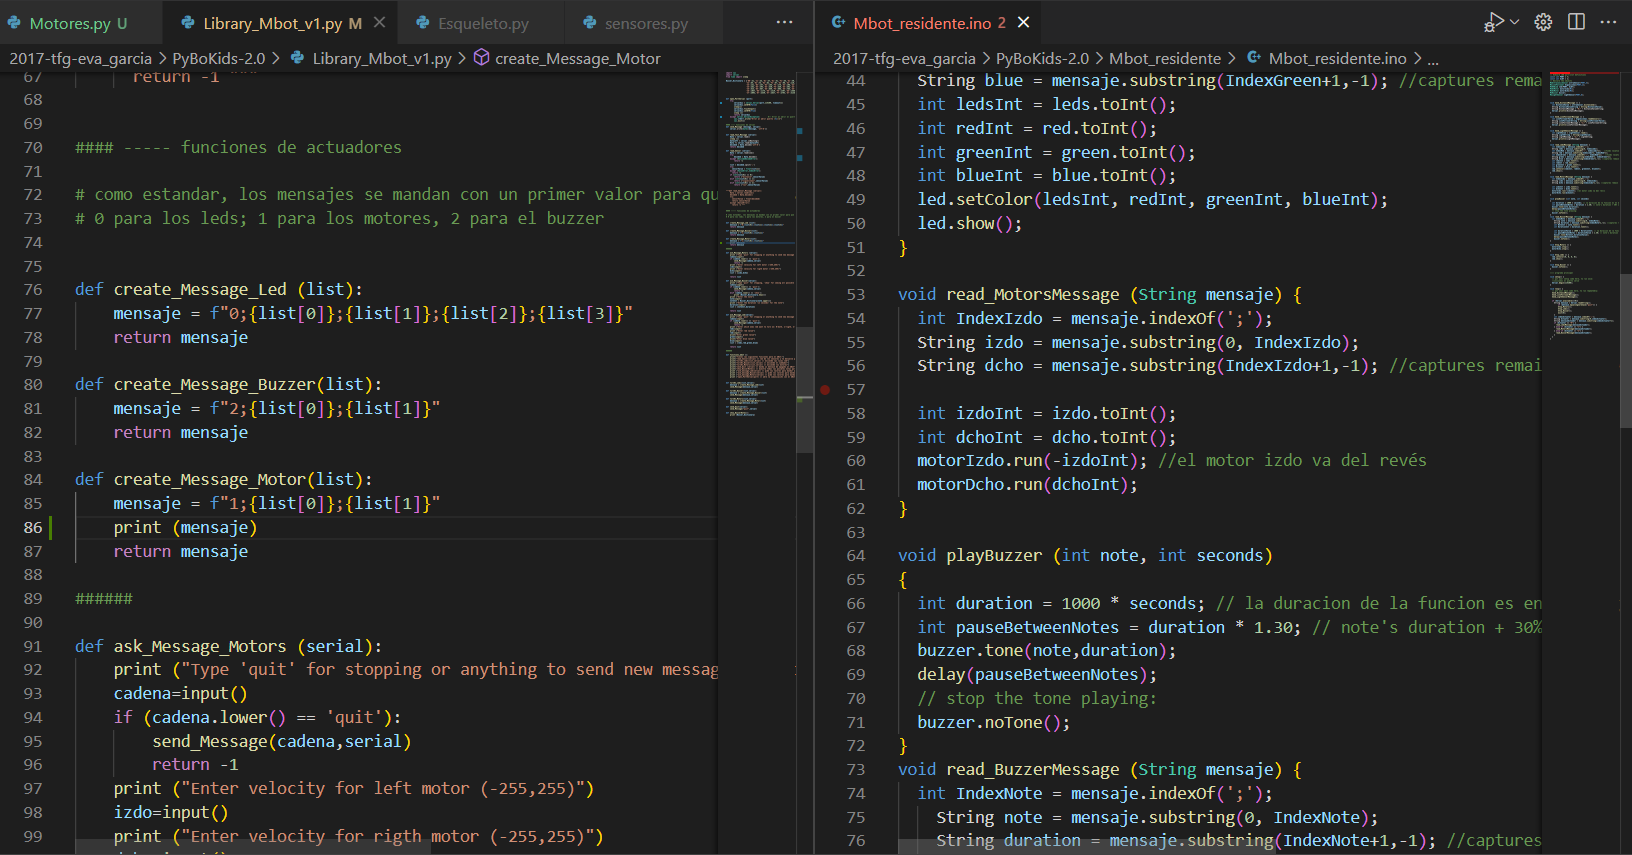
\includegraphics[scale=0.4]{programas.png}
	\label{img:Mix}
	\caption{Programa PC y Residente}
\end{figure} 
\vspace{1cm}
Utilizaremos como ejemplo de uso de las bibliotecas un ejercicio simple, utilizado durante el proceso de desarrollo de las bibliotecas, en el que se piden por pantalla las velocidades para los motores, y se manda el mensaje al programa Residente.\\
En este ejemplo, el programa principal tiene el siguiente código:
\begin{lstlisting}[language=python,caption={Ejemplo de uso de PyBoKids 2.0},captionpos=b]
import serial
from time import sleep
from Library_Mbot_v1 import *

print ("Usar los motores (M1 y M2) componiendo el mensaje completo para mandar exactamente los valores")
serial = open_PortSerial('com3')

while True:
	try:
		print ("Send new message or quit?")
		cadena=input()
		if (cadena.lower() == 'quit'):
			send_Quit(serial)
			break
		print ("Enter velocity for left motor (-255,255)")
		izdo=input()
		print ("Enter velocity for rigth motor (-255,255)")
		dcho=input()
		turnOn_Motors([izdo,dcho],serial)
	except KeyboardInterrupt:
		send_Quit(serial)
		break

serial.close()
\end{lstlisting}

Para visualizar el correcto funcionamiento del mensaje, imprimimos el mensaje, codificado, por pantalla. Aunque este código de depuración no estuviera en la versión final de la biblioteca de Python, sí ha sido útil y necesario durante el proceso de su desarrollo:

\begin{lstlisting}[language=python,caption={Uso de la bibliotca durante su desarrollo, con depuración de código},captionpos=b]
	def create_Message_Motor(list):
		mensaje = f"1;{list[0]};{list[1]}"
		print (mensaje)
		return mensaje
\end{lstlisting}

\begin{figure}[h]
	\centering
	\includegraphics[scale=0.6]{ejemploEjercicio.png}
	\label{img:ProgramaPrincipal}
	\caption{Programa Principal}
\end{figure} 
 
El Programa Residente, recibe el mensaje, lo decodifica y extrae el identificador '1' correspondiente a los motores, por lo que llama a la función que separa el resto del mensaje para obtener los valores de velocidad y lo envía al actuador:

\begin{figure}[H]
	\centering
	\begin{subfigure}
		[Extraer el identificador]{
			\includegraphics[width=0.45\textwidth]{ejemploEjercicio2.png}
			\label{img:ejemplo2}}
	\end{subfigure}
	\begin{subfigure}
		[Decodificar mensaje completo]{
			\includegraphics[width=0.5\textwidth]{ejemploEjercicio3.png}
			\label{img:ejemplo3}}
	\end{subfigure}
	\label{img:ProgramaResidente}
	\caption{Programa Residente}
\end{figure}

El resultado real puede verse en las siguientes imágenes, y el proceso completo en el \href{https://www.youtube.com/watch?v=GbFC0OJPLk0}{siguiente vídeo}.


\begin{figure}[H]
	\centering
	\begin{subfigure}[b]
		[Ejecución programa Principal]{
			\centering
			\includegraphics[scale=0.7]{ejemploEjercicio4.png}
			\label{img:ejemplo4}}
	\end{subfigure}
\newline
	\begin{subfigure}[b]
		[mBot]{
			\centering
			\includegraphics[scale=0.5]{ejemploEjercicio5.png}
			\label{img:ejemplo5}}
	\end{subfigure}
	\label{img:Resultadoexperimental}
	\caption{Resultado experimental}
\end{figure}
	\chapter{Aplicación robótica educativa}\label{cap:aplicationEducativa}
En este capítulo proporcionaremos una propuesta educativa  basada en ejercicios prácticos, cuyo objetivo global es el aprendizaje de robótica y pensamiento computacional, y de sus principios y conceptos básicos. \\
Estos ejercicios prácticos utilizan dos herramientas diferentes, cuyo orden temporal es fijo por lógica educativa: la primera herramienta, Scratch, la nativa del fabricante del robot mBot, es más sencilla al no ser un lenguaje de programación al uso. Una vez superada la primera fase de aprendizaje, será posible pasar a un lenguaje de programación de texto con sintaxis, compilación, ejecución por comando, etc, utilizando Python y la plataforma diseñada en este Trabajo Fin de Grado. 
\section{Enseñanza de robótica y programación con robot mBot}
Con el objetivo de enseñar pensamiento computacional y programación a jóvenes y de provocar un interés a corto y largo plazo en ello, la robótica es el encuadre perfecto. Utilizando una herramienta que contemplan como un juego, seremos capaces de guiarles en conceptos aparentemente complejos, programación, algoritmia, etc, de forma intuitiva y simple, sin entrar en compleja teoría que les haría perder la atención e interés. El robot elegido y las herramientas software utilizadas y previamente explicadas, componen un marco lo suficientemente simple para ser utilizado sin problemas y sin necesidad de conocimientos previos, proporcionando a la vez suficiente capacidad para las enseñanzas y objetivos perseguidos.

 
\subsection{Contexto}\label{subsec:contexto}
Los ejercicios de Scratch explicados a continuación no son el resultado de un diseño meramente teórico, sino que fueron puestas en práctica durante un curso completo, en el marco de unas clases extraordinarias de robótica, a alumnos y alumnas de Educación Primaria en el colegio Nuestra Señora de Rihondo, en Alcorcón (Madrid). Pudo comprobarse la acogida y la efectividad de los contenidos, en algunos casos adaptando la dificultad o añadiendo pasos a la primera versión del ejercicio si fuera necesario. \\
La plataforma Python original, PyBoKids (ver en \cite{JdeRobot}), requería de una instalación de JdeRobot y el simulador Gazebo, compleja, en Linux. Durante el curso escolar, se comprobó que esta era poco adaptable a un curso  completo de alumnos. Para este Trabajo Fin de Grado diseñamos por tanto, una versión de la plataforma que poder usar fácilmente en un contexto de clase colectiva. No es necesario instalar nada, aparte de Python, en los equipos (normalmente equipos de escuela, de prestaciones limitadas). De hecho, dado que el residente completo va grabado en el robot y no es necesario cambiar el programa grabado cuando se quiera usar una práctica diferente, no es necesario instalar siquiera Arduino. Sólo será necesaria la instalación de Python y el archivo \textit{.py} correspondiente a la biblioteca de PyBoKids-2.0 \\
Las prácticas descritas para la segunda parte son una transcripción de algunas prácticas de Scratch (las relativas a aplicaciones), adaptadas a los periféricos disponibles en PyBoKids-2.0 y con las limitaciones físicas que conllevan tener el robot conectado por cable al PC (para mantener la comunicación entre Python y el canal Serial). 


\subsection{Metodología}\label{subsec:metodología}
Las metodologías de cualquier tipo de programación son perfectamente utilizables en robótica y en el trabajo con jóvenes. La más intuitiva de ellas, de hecho la que ellos mismos utilizan de una forma natural (aunque no completamente ordenada), es \textit{Agile}\footnote{Filosofía de Desarrollo web basada en iteraciones}. Sin embargo, a los estudiantes no les explicaremos explícitamente que estamos usando este método, sino que diseñaremos los ejercicios con el fin de que deba usarse, y les guiaremos durante la ejecución con este método. 
\begin{figure}[h]
	\centering
	\includegraphics[scale=0.3]{agile.png}
	\label{img:agile}
	\caption{Esquema de una iteración Agile}
\end{figure}
Aunque las etapas de una iteración Agile clásica son cinco (\textit{Plan, Diseño, Desarrollo, Test y Feedback}), al ser Scratch y las prácticas un entorno muy sencillo, haremos con éstas un Agile simplificado, fusionando las fases de Plan y Diseño, que con los alumnos serán trabajo común. Las fases de Test y Feedback no las fusionaremos propiamente, sino que las haremos a la vez y poniendo las ideas en común: probando el ejercicio en el robot y comprobando si el comportamiento es el deseado. \\
Durante las clases, la metodología será de trabajo en común para el planteamiento del ejercicio, e individual (o por parejas dependiendo del ratio de robot por persona) para el desarrollo y el test.
\section{Programación robótica con Scratch}\label{sec:scratch}
Las prácticas de esta etapa están pensadas con unos objetivos docentes individuales, y otros globales con respecto al curso completo de ejercicios. Además, no podemos perder de vista que, para los estudiantes, las clases de robótica deben ser \textit{entretenidas}; dado que no son curriculares es importante mantener su atención creando ejercicios dinámicos y diferentes cada vez, además de con contenido educativo. 
\subsection{Makeblock}\label{subsec:makeblock}
Antes de pasar a describir las prácticas diseñadas, hablaremos de la plataforma nativa para la programación del robot mBot \textbf{mBlock}, del fabricante Makeblock (ver en \cite{makeblock}), y cómo lo utilizaremos en las clases. \\
Como hemos adelantado en el Capítulo \ref{cap:infra}, donde explicamos su instalación y uso básico, el fabricante pone a disposición un aplicativo, disponible para PC y dispositivo móvil (o tablet), para programar el robot mBot (y todos sus modelo de robot) con el lenguaje Scratch de una forma muy intuitiva. Este software es muy útil para la programación con jóvenes sin experiencia: requiere solamente de la instalación del software, y tiene integrados la forma de conectar con el robot y de grabar el código de un programa en la placa.
\begin{figure}[h]
	\centering
	\includegraphics[scale=0.5]{mblock_ejemplo.png}
	\label{img:pantallamblock}
	\caption{Aplicación mBlock: pantalla inicial}
\end{figure}

En nuestro caso, lo utilizaremos durante las clases en la primera parte del curso, orientada a la solución de los ejercicios con Scratch. 
Para ello, el propio alumno/a hará el proceso inicial de actualización de firmware, sólo necesario una vez, y de conexión mBlock-Robot (esta, sin embargo, será necesaria cada vez, puede verse en el propio programa si el robot está conectado o no). Este procedimiento está explicado en la sección \ref{list:conexionMblock}. \\
El proceso de solución de un ejercicio utilizando Scratch y mBlock, siguiendo los objetivos Agile marcados, es el siguiente:
\begin{enumerate}
	\item Discusión sobre el problema planteado, toma de requerimientos común.
	\item Diseño de un esquema de solución con soporte visual (pizarra), y separación del problema completo en pequeños ejercicios unitarios (\textit{bottom-up}).
	\item Programación en Scratch del primer problema unitario.
	\item Grabación en el robot del programa (ver en las imágenes \ref{img:uploadArduino1} y \ref{img:uploadArduino2}) diseñado. Para grabar el programa, será necesario que el robot esté conectado por USB al PC, encendido y establecida la conexión entre PC y mBlock.
	\item Prueba de la solución unitaria. Para ello, podemos desconectar el robot, ya que el programa está grabado en la placa (no hay ningún programa ejecutando en el PC que requiera mantener la conexión). Es notable el hecho de que, nada más subir el programa a la placa, comenzará a funcionar. Para poder ejecutar el programa ''desde cero en limpio'', podremos apagar el robot una vez hayamos grabado el programa, y volverlo a encender donde o cuándo queramos probar la solución. La placa Arduino ejecutará el programa que tenga grabado desde cero cada vez que se encienda, hasta que otro programa sea grabado.
	\item Continuación hasta la solución completa.
\end{enumerate}
\subsection{Prácticas con actuadores} \label{subsec:practicasactuadores}
 Como se ha explicado anteriormente, el propósito de un actuador es ejecutar la orden que recibe de la placa. Es, por tanto, muy visual y conveniente para introducir el curso de robótica, pues da pie a equivocarse y aprender de los errores de forma mucho más intuitiva que con otros componentes.
  
\begin{description}
\item [Carreras]\label{ej:carreras}
Obviamente, lo más visual del robot Mbot son los motores. También es lo más intuitivo y esperable de un robot en general: que se mueve por sí mismo. Es uno de los componentes más sencillos de programar, ya que Scratch ofrece un desplegable con los posibles valores que aceptan los motores del Mbot. Además, tiene métodos directamente para avanzar, retroceder y girar, muy cómodos para el primer contacto con el robot y válidos para este ejercicio en concreto. \\
En vez de simplemente \textit{mover} el robot, el ejercicio se pensó como una carrera entre los robot de todos los alumnos, para despertar su interés y hacerlo más entretenido; sin una utilidad práctica, o un juego, los alumnos perdían interés rápidamente o, incluso, no lo tenían desde el principio. \\
\textbf{Ejercicio Extra} Otro punto que se pudo comprobar con la experiencia empírica es que era mejor hacer varias versiones de un mismo ejercicio, aunque la dificultad fuera la misma, con objetivos distintos. Los alumnos no pierden la atención y aprenden que una misma solución, con pequeñas variaciones, vale para distintas situaciones. Además, así queda cubierta la situación de que los alumnos vayan a distintas velocidades y unos terminen el ejercicio base mientras otros no.\\
Otra versión de este ejercicio de carreras es hacerla con obstáculos fijos. Los alumnos tendrán que medir en tiempo la distancia entre obstáculos y jugar, con las velocidades y los giros. Quién mejor combinación encuentre, mejor tiempo hará en carrera.\\
Con este ejercicio, con sus diferentes versiones de obstáculos y de distancias, introducimos el concepto de actuador, explicando en clase la definición, y también el concepto de robot (primer concepto que se comentará y al que volveremos repetidamente durante el curso para revisar la definición que den los estudiantes). También el concepto de ''programación secuencial temporal'', ya que para evitar los obstáculos deberán programar Scratch para avanzar durante \textit{x} tiempo, después girar, volver a avanzar, etc.

\begin{figure}[H]
	\centering
	\includegraphics[scale=0.6]{carreras.png}
	\label{img:carreras}
	\caption{Ejemplo de solución para las carreras}
\end{figure}

\begin{figure}[H]
	\centering
	\includegraphics[scale=0.6]{carrerasrobot.png}
	\label{img:carrerasrobot}
	\caption{Uso en clase del ejercicio de carreras}
\end{figure}

\item [Cumpleaños feliz]\label{ej:cumple}
Otro actuador sencillo de usar es el zumbador integrado en la placa. Es algo más complicado, pues las notas musicales no son las más conocidas y, sobre todo en los alumnos más jóvenes, no están acostumbrados a una escala musical. Sin embargo, se puede comprobar que no tardan mucho en entender el sistema de escalas; se les ayudará dándoles la tabla de equivalencias entre las notas americanas y europeas (ver en el cuadro \ref{table:notas}).
\begin{table}[H]\centering
	\begin{tabular}{||ccccccc||}
		\hline
		Do & Re & Mi & Fa & Sol & La & Si \\[1.5pt]
		C & D & E & F & G & A & B \\
		\hline
	\end{tabular}
	\caption{Equivalencia entre notas}
	\label{table:notas}
\end{table}

Una vez entendida la diferencia de notas y comprobado cómo funciona el zumbador, les proponemos que el robot entone la canción de cumpleaños feliz - o cualquier otra 	que seguro conozcan-. No sólo sirve para el actuador, sino que introducimos el concepto de repetición (bucles). La idea principal es dejarles al principio que hagan el ejercicio todo seguido y después les ayudamos a entender que están repitiendo código: hay estrofas que se repiten. Ven la necesidad, pues, de meter esas estrofas dentro de un bucle de repetición de tantas veces como sea necesario.\\
\textbf{Ejercicio Extra}. Una vez han terminado la primera canción, es bueno invitarles a que intenten que el robot \textit{cante} otras melodías que conozcan y les apetezcan.

\item [S.O.S.]\label{ej:sos}
El siguiente actuador del pack del mBot son las luces LED de la placa, el rango de colores RGB permite que cada alumno pueda personalizar los colores como más les guste. El propio lenguaje Scratch permite el rango de cada color entre 0 y 255 (aunque en la práctica, no sean notables los cambios pequeños en esa escala).\\
La finalidad del ejercicio es que, con luces, el robot pida ayuda en lenguaje morse: tres pulsos cortos, tres pulsos largos, y tres pulsos cortos. \\
Como se ha comentado anteriormente, los alumnos son más proactivos cuando ven una utilidad mínimamente real a lo que se les pide, y conocen el lenguaje morse -o es muy sencillo de explicar- y la utilidad de pedir ayuda en un lenguaje universal.\\
En este ejercicio reforzamos las duraciones; el progreso temporal de las órdenes. Los puntos y rayas del morse los traducimos a esperas de menos y más tiempo, respectivamente. También reforzaremos el concepto de bucle, pues el mensaje podremos repetirlo con un bucle en vez de repitiendo todas las órdenes. En \href{https://www.youtube.com/watch?v=k6QSnIkRVyo}{este vídeo} podemos ver el resultado de hacer el ejercicio en clase y en la figura \ref{img:SOS} un ejemplo de solución propuesta.
\begin{figure}[h]
	\centering
	\includegraphics[scale=0.8]{SOS.png}	
	\caption{Ejemplo de solución para el mensaje SOS en morse}
	\label{img:SOS}
\end{figure}
\textbf{Ejercicio Extra}. Una vez que han conseguido que el mensaje de socorro sea entendible, cambiamos el ejercicio a escribir en morse cualquier mensaje que se les ocurra (con la tabla de equivalencias del abecedario) y a mandar el mismo mensaje de socorro con luz y sonido a la vez.
\item[Camión]\label{ej:camion}
Como último ejercicio de actuadores, intentaremos juntarlos todos, a la vez que todavía no introducimos ningún sensor. Proponemos, pues, emular el comportamiento de un camión, algo a lo que están acostumbrados y que no se les habría ocurrido que era automatizable. Un camión, haga lo que haga, si da marcha atrás, pitará (con los zumbadores) y encenderá las luces naranjas. \\
Vamos metiendo, poco a poco, acciones simultáneas, para que tengan que preocuparse de más de un componente (de más de un bloque de Scratch). El objetivo es el aprendizaje de que, en robótica, un comportamiento aparentemente trivial es la suma de muchos comportamientos simultáneos y dependiente uno de otro.\\
Con este ejercicio aprendemos el concepto, tan necesario en la programación de robótica, de \textit{concurrencia}. Cuándo, y sólo cuándo, el camión da marcha atrás, es cuando se encienden las luces y sirenas.
\end{description}

\subsection{Prácticas con sensores} \label{subsec:practicassensores}
Como se ha comentado en el Capítulo \ref{cap:infra}, los sensores recogen información del medio y la devuelven en forma numérica. Es misión del programador, pues, procesar el retorno y la interpretación de esa información de forma correcta, unívoca y cubriendo todos las posibilidades. \\
Esto requiere unas habilidades más avanzadas, además de los conceptos básicos de programación como bucles, condicionales, ocurrencias, etc, que se han visto en los ejercicios anteriores de actuadores. Los alumnos deberán ser capaces de:
\begin{enumerate}
	\item Decidir qué información necesitan del entorno para el problema que se les presenta. Es decir, dividir el problema en pequeños trozos hasta llegar al más pequeño de ellos. Éste será del que tengan que abstraer el tipo de información que necesitan conocer para poder solucionarlo.
	\item Una vez conocida la información que necesitan, deberán elegir qué sensor es el que mejor les va a dar como respuesta esa información. Al principio, será una cuestión trivial, pues sólo habrá una posibilidad, pero después introduciremos ejercicios que requieran de varias \textit{informaciones} distintas, por lo cual, de varios sensores.
	\item Tras obtener del sensor el valor de retorno numérico, es misión del alumno diseñar la respuesta de vuelta del robot, es decir, cómo deba comportarse dependiendo de esa respuesta. No será lo mismo si queremos acercar el robot a un muro lentamente para aparcar, que si debemos tener cuidado de que no choque o si debe perseguir a otro robot: el sensor es el mismo, y el valor de retorno también, pero el comportamiento no tiene por qué ser el mismo. 	
	\item Fijándose en la necesidad original, y en las repuestas que se reciben de cada sensor, deberán ser capaces de granular la sensibilidad del sensor, o del valor de control, para obtener un comportamiento lo más refinado y preciso posible (siempre teniendo en cuenta las limitaciones técnicas del mBot).
\end{enumerate}

Estas habilidades las iremos trabajando poco a poco, diseñando ejercicios que las introduzcan a la vez, pues son necesarias todas, pero con diferentes niveles de dificultad.\\
Como siempre, en cada ejercicio iremos guiando a los alumnos en la división del problema de forma \textbf{bottom-up}; esta división de los problemas es una de las habilidades más importantes en programación, y una de las cosas sobre las que más haremos hincapié.

\begin{description}
	


\item [No chocar contra un muro]\label{ej:muro}
Uno de los actuadores más visibles, y por el que los alumnos siempre preguntan, es el sensor de proximidad (sensor de ultrasonidos). El bloque de Scratch para este sensor devuelve un valor numérico, la distancia a la que se encuentra del obstáculo que esté leyendo. Por tanto, para los alumnos es tan cómodo como trabajar con ''distancia x del sensor''. \\
Este ejercicio se diseñó con el mismo ánimo que el del camión (\ref{subsubsec:camion}), siguiendo la idea de que programen cosas que conocen, que utilizan en su día a día, con el fin de que aprendan la idea que la robótica es algo que está incluida en nuestras vidas y cualquiera puede dedicarse a ello.\\
El objetivo es, por tanto, programar el sensor de proximidad de los coches, que cuando aparcan y se acercan al coche de delante (en este caso, a un muro), primero pita, si te acercas más pita más rápido y, al final, se para. \\
Como es el primer sensor que utilizan, lo orientaremos en etapas. \\
Primero, necesitan aprender cómo se usan el sensor y el valor de retorno. Es decir, el bloque de Scratch que llama al sensor no sirve de nada sin añadirlo a algún otro bloque que utilice el valor que el sensor lee del entorno (por ejemplo, un bloque condicional). Este primer ejercicio lo haremos utilizando directamente el bloque de lectura del sensor; más adelante introduciremos el concepto de variable.\\
Después, tendrán que conseguir la parte difícil del ejercicio: que el robot se pare cuando se acerque al muro. Así comprobarán de forma real cómo funciona el sensor, además de ajustar la sensibilidad de ''cuánto de cerca'' debe estar el robot para considerar que está pegado al muro pero para qué dé tiempo a pararlo sin que se choque.\\
Una vez conseguida esta primera parte, que requiere de bloques condicionales, de ocurrencia o de espera (no hay una sola forma correcta de hacerlo), solucionar el ejercicio completo es -relativamente- inmediato. Como se ha explicado antes, el comportamiento deseado es que, cuando el robot se acerque un poco al muro, pite ligeramente (con el zumbador de la placa, que ya se ha utilizado antes; véase \ref{ej:cumple}); cuando se acerque algo más, pite más intensamente y, cuando esté muy cerca (la distancia que se haya decidido en la primera parte del ejercicio), parará para no chocar.
\textbf{Ejercicio extra}. Siempre podemos refinar algo más el ejercicio para que, además de pitar, el robot vaya disminuyendo la velocidad según se acerque al muro hasta, finalmente, pararse. Esto sería una aproximación un poco más cercana al aparcamiento autónomo que llevan incorporado algunos de los coches más modernos.\\
Como ampliación, este ejercicio puede adaptarse para meter la funcionalidad secundaria dentro de \textbf{funciones} (en Scratch, nuevo bloque), con un parámetro de entrada del que dependerá la velocidad o la frecuencia de pitido. Estas funciones serán llamadas más tarde, desde el programa principal, con el parámetro de entrada correspondiente a cuánto de cerca esté el robot de la pared. Obviamente, esta funcionalidad no la podremos introducir nada más empezar con los sensores. La experiencia nos demuestra que es mejor esperar a que sean los propios alumnos los que creen las necesidades, y la necesidad de una \textit{función} no la verán hasta que no tengan programas muy grandes (con muchos bloques) y difíciles de leer; será entonces cuando ellos mismos pidan de forma natural paquetizar el código.\\
Esta ampliación la reservaremos, por tanto, para retormarla cuando hayamos visto otro ejercicio en el que sí se necesiten las funciones. Como los alumnos guardan los escenarios con el código de los ejercicios, será fácil retormarlo para cambiarlo.

\item[Luces automáticas]\label{ej:lucesAuto}
En este ejercicio, utilizaremos el sensor de luz, también integrado en la placa. Siguiendo la idea de 'programar comportamientos de la vida diaria', en este caso desarrollaremos el sistema de las luces de un coche. Éstas se encienden automáticamente cuando no hay luz, bien porque fuera de noche, bien porque fuera un día nublado. Es decir, que si sólo programáramos las luces para que se encendieran a partir de las 8 de la noche, porque es la hora a la que en verano debiéramos encender las luces, en invierno estaremos horas sin luz pues anochece mucho antes. Por tanto, necesitaremos un sistema que nos valga siempre, no dependiendo de la hora a la que anochezca o de si el día es nublado o despejado. \\
Este ejercicio es muy simple por naturaleza, así que lo utilizaremos para introducir un método de cálculo del valor de referencia de la luz ambiental:
al principio del ejercicio, hemos comprobado el nivel de luz ''a mano''. Si cambiamos el sitio, o cualquier otro factor, habrá que volver a sacar este nivel barrera. Para tener que evitar hacer esto, metemos la comprobación en el programa principal, al principio del código. \\
El nivel de luz ambiente que se usará como nivel umbral se obtiene leyendo el nivel de luz del sensor durante \textit{n} veces (10, por ejemplo), sumándolos y dividiéndolos entre \textit{n}; es decir, se hace una media aritmética básica de todos los niveles de luz que se hayan leído. En Scratch, se meterá en un bucle el lector del sensor, combinándolo con esperas para coger valores diferentes, y se irá sumando en una variable (a sí misma); después se dividirá ente el número de veces que se hayan dado vueltas al bucle. A partir de calcular este valor umbral, se programará el robot para que, si apagamos las luces, se enciendan los LED de la placa (que sería el equivalente a las luces del coche).\\
Esta ampliación del ejercicio nos sirve para explicar el modo correcto de establecer 'variables de entorno'. Es decir, el entorno tiene unas características, que casi nunca serán fijas o deterministas y que se necesitan como datos para un desarrollo más sólido frente a errores o cambios en el entorno. Además, también servirá para aprender el concepto de \textbf{variable} de programación. Una variable es una ''caja'' donde se guarda un valor que vamos a querer utilizar más tarde. En este caso, el valor de la suma de las lecturas consecutivas del lector.\\
Este método de establecer el entorno en variables que se vayan a utilizar y, sobre todo, la necesidad de ello, se volverá a trabajar, con el ánimo de consolidar lo aprendido, en el siguiente ejercicio. 

\item[Huye-luz]\label{ej:huyeLuz}
Esta vez, y no como ejercicio extra sino como uno distinto, diseñamos otro problema con el mismo sensor que ya hemos utilizado en el anterior. El motivo de que sea un ejercicio diferente es que no es un añadido al ejercicio, sino que cambia el requerimiento inicial del problema; éste será que el robot huya de la luz, persiguiéndolo con una linterna.\\
Utilizaremos el mismo método de sacar el valor umbral de referencia pero, esta vez, si estamos por encima de ese valor (en vez de por debajo como antes), el robot tendrá que huir, dando marcha atrás y girando.\\

\item[Sigue-líneas]\label{ej:sigueLineas}
El siguiente sensor del robot es el sensor infrarrojo.
Utilizaremos, al principio, el circuito para seguir las líneas que viene en el kit del mBot, que hace un ocho con líneas negras sobre blanco. Es importante que cualquier otro circuito qe vayamos a hacer seguir al robot tenga claramente diferenciados el negro y blanco, pues el sensor es binario: está ''tapado'' o no, y si el suelo es oscuro entenderá que es una línea, y se comportará de forma errónea.\\
El objetivo del ejercicio es, obviamente, que el robot siga, sin ninguna interacción humana, el circuito sin salirse de las curvas. Para los alumnos más jóvenes, atacar este problema directamente resulta demasiado grande y no sabrán como empezarlo sin una guía para aprender a usar el sensor. Lo más difícil de este sensor, en comparación con los otros, es el concepto de \textit{respuesta binaria}. El bloque de Scratch permite acceder a este sensor y darle dos opciones: sensor en negro o sensor en blanco. El primer ejercicio sería, entonces, saber qué significa que el sensor responda negro o blanco (por ejemplo, que encienda las luces), tapándolo y destapándolo, lo que será equivalente a que esté sobre la línea negra o no.\\
La siguiente dificultad es pensar en las diferentes combinaciones de sensor derecho e izquierdo con el blanco y negro. En programación clásica, las combinaciones serías 00, 01, 10, 11, pero esto no vale en Scratch ni para los alumnos. Tendrán que decidir, con el robot y el circuito delante, qué significa cada posibilidad:
\begin{itemize}
	\item El sensor derecho sea negro y el izquierdo negro: está encima de la línea.
	\item El sensor izquierdo sea negro y el derecho blanco: se ha desviado hacia la derecha (o está en una curva a izquierdas).
	\item El sensor derecho es negro y el izquierdo blanco: se ha desviado hacia la izquierda (o está en una curva a derechas).
	\item Los dos sensores leen blanco: se ha salido completamente de la línea.
\end{itemize}
A partir de separar y entender las posibilidades que tenemos con los sensores, el siguiente paso es decididr qué hacer en cada caso de los especificados; se hará programando cada posibilidad a la vez que se diseña la solución.
\begin{itemize}
	\item Si los dos sensores son negros y el robot está en la línea, deberá continuar avanzando sin cambios.
	\item Si el sensor izquierdo es negro pero el derecho no, y el robot está desviado a la derecha, o en una curva, tendrá que girar hacia la izquierda; es decir: seguirá la trayectoria de la curva.
	\item Del revés, si el robot está en una curva desviándose a la izquierda, tendrá que girar a la derecha para seguir la curva.
	\item Si el robot lee los dos sensores en blanco, es que se ha salido del circuito y tendrá que volver a él (girando o dando marcha atrás hasta que el sensor vuelva a ser negro).
\end{itemize}
Una vez solucionado el ejercicio, sólo quedará perfeccionarlo haciendo los giros más precisos para que el movimiento sea más fluido y continuo. La primera vuelta de este perfeccionamiento se hará ajustando las velocidades y las esperas. La segunda vuelta, la forma más correcta de hacerlo, será siguiendo la idea de ''girar hasta estar en el sitio correcto''; es decir, que mantendremos el movimiento deseado (el correspondiente a cada caso), hasta que los dos sensores lean negro y esté otra vez sobre la línea.\\
Como puede observarse, este ejercicio es un ejemplo perfecto de iteraciones Agile.

\begin{figure}[H]
	\includegraphics[width=6cm]{mBotSigueLineas.jpg}
	\centering
	\label{img:mBotSigueLineas}
	\caption{Ejercicio de Sigue Líneas}
\end{figure}

\textbf{Ejercicio extra}. Esta vez no aumentaremos la dificultad ni cambiaremos o ampliaremos las especificaciones del problema, sino que sólo lo pondremos a prueba con diferentes circuitos hechos por los alumnos, cada vez más difíciles o con más curvas, con el fin de demostrar que con una única solución tenemos cubiertos todos los escenarios en todas las situaciones que planteemos. \\
Además, sirve para jugar con el programa que los alumnos han desarrollado, haciéndoles ver que sirve para algo más que sólo 'hacerlo'; es importante inculcarles la idea de que programar es divertido y de que ver los resultados es gratificante.

\item{Choca-gira}\label{ej:chocaGira}
Usaremos el mismo sensor de ultrasonido que en el ejercicio del muro (\ref{ej:muro}) pero complicando el requerimiento principal. Esta vez, en lugar de sólo tener que parar para no chocar, el robot intentará evitar el obstáculo para huir de él. \\
El ejercicio básico consistirá en perseguir al robot, poniéndole delante algo con que, de no esquivarlo, chocaría. Para esquivarlo, no sólo tendrá que parar si 'lee' un obstáculo delante sino que, deberá girar o dar marcha atrás o las dos cosas: serán los alumnos los que diseñen su propio algoritmo de \textbf{esquivado}; no hay una solución única y deberán demostrar su capacidad de decisión delante de una solución abierta. \\
\textbf{Ejercicio extra}. Con el mismo sensor y la misma filosofía que anteriormente, esta vez diseñaremos un algoritmo para \textbf{atravesar} los obstáculos y poder continuar la carrera, no para evitarlos y huir de ellos. \\
El propósito es reforzar la autonomía de los alumnos a la hora de buscar una solución, no sólo de implementar un algoritmo (una solución) dado. La diferencia con la carrera de obstáculos del primer apartado de este mismo capítulo, en \ref{ej:carreras}, es que la disposición de estos obstáculos no será fija, sino que el robot deberá ser capaz de solucionar cualquier circuito.
\end{description}

\subsection{Prácticas de aplicaciones}\label{subsec:practicasaplicaciones}
En las dos secciones previas se ha explicado cómo utilizar los sensores y actuadores propios del mBot con el lenguaje de programación Scratch, y se han propuesto ejercicios para practicar todos ellos. Sin embargo, y aunque siempre se ha intentado hacer estos ejercicios lo más reales posibles, a la hora de ponerlo en práctica podemos ver que los alumnos los superan fácilmente y que, en cuanto tienen resuelto el algoritmo, piden opciones que hacerle o le buscan formas distintas con las que poder jugar con el robot. \\
Con ese propósito, para la última parte del curso de Scratch, y ya teniendo en cuenta las herramientas de programación trabajadas hasta ahora, en esta sección propondremos algunos ejercicios más completos y que requerirán de varios sensores y actuadores conjuntos, con comportamientos más complejos y con un propósito más específico. Seguiremos trabajando la programación, reforzando los conceptos de \textit{funciones, variables, orden secuencial, ejecuciones bloqueantes, bucles anidados a condiciones, etc}. \\
Otro propósito de esta sección es el aprendizaje y autonomía de los alumnos a la hora de solucionar un problema. Es decir, no ya de dar la solución programada a un algoritmo, sino de diseñar ellos mismos ese algoritmo que compone la solución. A base de intentos, y distintas iteraciones, el refinamiento de la solución será un punto importante. Seguiremos la idea de la metodología \textbf{Agile}: diseño, desarrollo, prueba, rediseño. A pesar de haber seguido este método durante todo el curso, ahora es cuando mejor se puede poner en práctica debido a la naturaleza más continua de los ejercicios (no durarán sólo un día o una iteración).

\begin{description}
	\item[Lucha de Sumo]\label{ej:sumo}
	Con este primer proyecto se pretende demostrar a los alumnos que son perfectamente capaces de programar comportamientos que pueden usarse de forma completa y única, sin ser necesariamente sólo una pequeña parte de un comportamiento más completo. Es decir, en el caso de las luces automáticas (\ref{ej:lucesAuto}) o del sistema de detección de muros (\ref{ej:muro}), los programas formaban parte de un comportamiento completo al que podríamos referirnos como 'comportamiento robótico de un coche'; no tenían una aplicación directa por ellos solos. Sin embargo, en este ejercicio que nos ocupa, el comportamiento se programará desde el principio y al completo, con el fin de que los alumnos puedan ver y jugar con un programa hecho por ellos de forma íntegra. \\
	El objetivo del juego es simular un combate de sumo en el que los robot serían los luchadores. Se juega dentro de un ring, si un robot se sale, pierde; un robot, para ganar, deberá sacar al otro del ring. \\
	Para perseguir al otro ''luchador'', utilizaremos el lector de distancia. Si no tenemos nada a \textit{x} distancia, haremos girar al robot y avanzar un poco, así hasta que (y el bloque de control es este 'hasta que') tengamos un obstáculo a menos de esa distancia \textit{x}, momento en el cual pararemos de girar e iremos en la dirección en la que está el obstáculo (el otro robot). Como el objetivo es sacar al otro robot del ring, pero no salir de él, si captáramos con el sensor de Sigue Líneas que una o las dos líneas están tapadas (en negro), mandaremos al robot parar. Si las dos líneas estuvieran en negro, y hubiera un obstáculo (un robot) muy cerca, significaría que hemos ganado. Si no, que tenemos que seguir buscando al contrincante.\\	
	Como se puede observar, en este ejercicio se tendrán que mantener muchos sensores y posibles variaciones a la vez, por lo que los alumnos deberán tener muy en cuenta todas las variantes y la posibilidad de que una combinación niegue a la otra. Por ejemplo, que el robot no se salga del campo es prioritario, así que esa condición deberán considerarla la primera, antes de considerar si tienen delante el otro robot. Es decir, esa condición es bloqueante para considerar el resto.\\
	Como todas esas condiciones serán bloques de condición anidados, el código enseguida se haría ilegible, por lo que ahora más que nunca, es imprescindible utilizar funciones. Cada función será un comportamiento predefinido y que siempre será igual. Estas funciones serían las siguientes:
	\begin{itemize}
		\item No salirse del campo. El robot siempre hará lo mismo cuando se encuentre una de las líneas que delimitan el campo. Tendrá las dos opciones, que tenga un obstáculo delante, o que no. Con cada una de estas opciones, tendrá un comportamiento.
		\item Correr hacia la pelota. En cuanto el robot detecte, a una distancia predefinida, que el contrincante está delante suya, correrá más rápido, y siempre a la misma velocidad. 		
	\end{itemize} 
	Además, todos esos valores \textbf{constantes}, como las distintas velocidades o la distancia a la que considerar que la pelota está cerca, siempre serán \textit{variables globales}, en vez de valores numéricos embebidos en el código.
	
	
	\item[Laberinto] \label{ej:laberinto}
	Siguiendo la misma línea e 'proyecto', y de integración de conocimientos, esta vez proponemos el diseño de resolución autónoma de un laberinto. \\
	Lo primero que debemos comentar es el algoritmo de resolución del laberinto, teórico, que implementaremos en código. Dado que la intención es la ''robotización'' del proceso, haciéndolo independiente de la acción humana, nos basaremos en una de las formas clásicas de resolución de laberintos: siempre seguir la pared que se tenga a la derecha (o a la izquierda, pero siempre el mismo lado). Es decir, para salir de un laberinto, deberemos seguir desde la entrada del mismo, la pared que tengamos a la derecha; en caso de encontrar un giro (una esquina) deberemos seguirla también. Este método se conoce como 'método de la mano derecha' y sirve para la mayoría de laberintos. En la siguiente imagen se observa con claridad:
	\begin{figure}[H]
		\includegraphics[width=3cm]{laberinto.png}
		\centering
		\label{img:laberinto}
		\caption{Método de la mano derecha}
	\end{figure}
	Este método no asegura el camino más corto sino la certeza de la resolución. De hecho, en la imagen puede observarse que si hubiéramos utilizado el método de la mano \textit{izquierda}, el camino habría sido más corto. Sin embargo, como el objetivo es utilizar un sólo método para todos los posibles laberintos, escogeremos uno e implementaremos todos los alumnos el mismo. \\
	Lo primero sería la preparación, del robot y del entorno. Como necesitaremos que el robot vea paredes a los lados, y no solo de frente, utilizaremos el sensor Sigue Líneas como 'lector de paredes'; adaptaremos al robot cambiando de lugar este sensor:
	\begin{figure}[H]
		\includegraphics[width=6cm]{mBotlaberinto.jpg}
		\centering
		\label{img:mBotlaberinto}
		\caption{Preparación del mBot}
	\end{figure}
	Esta necesidad de 'cambiar' al robot serán los propios estudiantes quiénes la verán, durante el proceso de toma de requerimientos, y después de haber conocido el algoritmo de la mano derecha. Para este proceso de preparación, será necesario haber montado un laberinto de pruebas, por ejemplo de porexpan (cualquier laberinto simple, el de la imagen por ejemplo). Verán la necesidad de conocer si hay una pared al lado o no, y si hay otra enfrente o no, cuando físicamente vean el robot dentro del laberinto e intenten resolver el algoritmo. \\
	Siguiendo el mismo procedimiento Agile que durante el curso, programaremos el comportamiento en etapas unitarias, en modo \textit{bottom-up}, y con su fase de test entre cada una (varias fases de test, de recalibración de velocidades, de perfeccionamiento, etc):
	\begin{enumerate}
		\item Idea principal del algoritmo: seguir la pared de la derecha. Para ello utilizaremos el sensor infrarrojo Sigue Líneas de forma que, si están los dos sensores tapados (negro) hay pared y debemos seguir avanzando; si están los dos sensores destapados (blanco) hemos pasado una esquina ''a derechas'' (sin tener pared delante) y tenemos que girar a la derecha \textbf{hasta que} los dos sensores vuelvas a estar tapados.
		\item Esta condición anterior es así \textbf{mientras que} el sensor de distancia delantero no tenga una pared a \textit{x} distancia. Si están los dos sensores infrarrojos tapados, pero tenemos una pared delante, significará que tenemos una esquina ''a izquierdas'' y deberemos girar hacia la izquierda \textbf{hasta que} no haya pared delante.
		
	\end{enumerate}
	El trabajo más importante para el estudiante será el diseño de 'estados' del robot; qué estados son bloqueantes (van antes en el código) y el orden en que analizar todas las variables disponibles.
	
	
	\item [Aparcamiento Autónomo] \label{ej:aparcamiento}
	Este ejercicio, muy interesante para los alumnos y alumnas por ser especialmente "real", es posible con la misma configuración de sensores que la del laberinto. El propósito es programar el comportamiento de un sistema de aparcamiento de un vehículo moderno, que cuando encuentra un hueco suficientemente grande, aparca de forma autónoma. Las distintas fases de diseño, serían las siguientes:
	\begin{enumerate}
		\item El primer problema que atajar es qué significará para el robot un sitio ''suficientemente grande''. La premisa del entorno será una 'pared' creada con porexpan, o algo equivalente, que en un momento determinado 'desaparece. Por tanto, utilizaremos el sensor lateral de forma parecida al ejercicio anterior: mientras que los dos sensores estén en negro, tendremos que seguir avanzando.
		\item Cuando los dos sensores laterales estén en blanco, significará que hemos encontrado un \textit{posible} hueco. Si es suficiente o no, como el robot no tiene capacidad de calcular su propio tamaño, vendrá determinado por cuánto tiempo avancemos (iniciando una variable tiempo a 0) \textbf{hasta que} los dos sensores vuelvan a estar tapados. El tiempo que tarde en encontrar un hueco suficientemente grande lo calcularemos una vez, y lo utilizaremos como valor referencia en el programa principal: si es mayor que \textit{T}, será suficiente, si no, hay que seguir buscando.
		\item Tras encontrar un hueco, el robot deberá parar y dar marcha atrás (girando ligeramente) \textbf{hasta que} el sensor delantero tenga un valor de referencia, lo que significará que tiene un 'coche' delante. 
		\item Este proceso puede perfeccionarse todo lo que los estudiantes quieran, para mejorar el aparcamiento y que sea más preciso.		
	\end{enumerate}
	Una variación interesante de este ejercicio, una vez que los estudiantes hayan programado el algoritmo, es cambiar la disposición de los sensores: poner en el lateral el sensor de distancia de ultrasonidos, y delante el infrarrojo. El procedimiento es el mismo, pero deberán ajustar los valores, re-calcular las constantes de referencia y re-diseñar los detalles de implementación. Lo más importante es que aprenden que las soluciones a un mismo problema no son únicas.
	\begin{figure}[H]
		\includegraphics[width=6cm]{mBotaparcamiento.jpg}
		\centering
		\label{img:mBotaparcamiento}
		\caption{Ejercicio de aparcamiento autónomo}
	\end{figure}
	Otra posible variación, útil en caso de que haya alumnos que trabajen a diferentes velocidades (algo muy habitual) es añadirle la funcionalidad trabajada en otros ejercicios, por ejemplo que emitiera sonido con la marcha atrás (\ref{ej:camion}).
\end{description}


\section{Programación robótica con Python: PyBoKids 2.0}\label{sec:Python}
Esta segunda parte del curso educativo está supeditada a que los alumnos hayan tenido una buena acogida de los contenidos de la primera etapa, tanto educativa como temporalmente. Es importante que hayan aprendido globalmente conceptos de programación para poder introducir el concepto de 'código', con todas las normas que ello conlleva. Scratch para ello es una ventaja frente a otros lenguajes ''infantiles'', pues es una suerte de \textit{pseudocódigo}, frente a otros que no contienen nada de texto y son completamente pictográficos (orientados a alumnos aún más jóvenes, que no han empezado o terminado de aprender a leer). \\
Se han diseñado pues, una serie de ejercicios de dificultad progresiva, para introducir a los estudiantes en la programación clásica y dar un paso más en su aprendizaje en robótica, utilizando la plataforma diseñada en este Trabajo Fin de Grado PyBoKids 2.0.
\subsection{PyBoKids 2.0}
El objetivo de la plataforma desarrollada es ofrecer una fórmula para que personas que no han utilizado nunca un lenguaje formal de programación, programen el robot mBot con ese lenguaje. El hecho en sí es complicado, ya que tiene varios hándicap que superar: la edad de los alumnos, la complicación de empezar a programar y además, de aprender un lenguaje de cero, sumada al hecho de estar utilizándolo para robótica, y no sólo programación ''básica''. Esta plataforma, pues, ofrece una posibilidad para no depender del lenguaje de la placa, Arduino, más complejo y menos manejable para la situación. \\
El uso en clase de  PyBoKids será muy sencillo:
\begin{enumerate}
	\item Los robot llevarán ya grabado el programa residente de Arduino, para que no sea necesario hacerlo en clase. Sin embargo, si un alumno u alumna quisiera hacerlo de forma independiente, el procedimiento de instalación está explicado en \ref{list:InstalacionArduino}. Será necesario: 
	\begin{itemize}
		\item Instalación del Arduino IDE
		\item Descargar las librerías de Arduino y el programa residente de \href{https://github.com/JdeRobot/PyBoKids/tree/main/PyBoKids%202.0}{aquí}
		\item Incluir las librerías según las instrucciones del Capítulo \ref{cap:infra} comentadas
		\item Abrir el fichero de extensión .ino del programa residente anteriormente descargado, y grabarlo en la placa
	\end{itemize}
	\item Descargar e instalar Python 3.0 según las instrucciones en \ref{list:instalacionPython}
	\item Descargar la biblioteca de PyBoKids (fichero \textit{Library\_mbot\_v1}) y el fichero \textit{esqueleto.py} desde \href{https://github.com/JdeRobot/PyBoKids/tree/main/PyBoKids%202.0}{el repositorio de PyBoKids 2.0}, y guardarla localmente en el directorio donde vayamos a trabajar.	
	\item Abrir el fichero \textit{esqueleto} y guardarlo con el nombre del programa que vayamos a realizar, para guardar una copia (y no sobreescribirlo).
\end{enumerate}

Como puede verse, el proceso es muy sencillo, y al alcance de los alumnos. 
\subsection{Prácticas de lenguaje}
Como sería la primera vez que utilizan un lenguaje de programación clásico, es necesario introducirlos en las normas, en la sintaxis básica y en la forma de ejecución. Para ellos hemos preparado unos ejercicios simples sólo de lenguaje, a los que dedicar poco tiempo (pues no son de robótica), a modo de introducción.
\begin{description}
\item [Hola mundo] Como en cualquier curso introductorio de lenguaje, el primer 'Hola mundo' es fundamental para enseñar a los alumnos a abrir un fichero nuevo, guardarlo, y ejecutarlo (en este caso, usaremos el IDLE nativo de python en Windows, al igual que su shell. Es por tanto, muy fácil ejecutar un programa guardado con la opción propia del IDLE).
	\begin{figure}[H]
		\includegraphics[scale=0.6]{hola.png}
		\centering
		\label{img:holamundo}
		\caption{Hola Mundo en Python}
	\end{figure}
\item [Calculadora] Para aprender cómo usar variables en Python, y como acceder a ellas, haremos algo tan simple como útil: guardar dos valores diferentes en dos variables, \textit{a} y \textit{b}, e imprimir por pantalla la suma, resta, multiplicación y división de ellas. 
\item[Calculadora II] El mismo ejercicio anterior, pero pidiendo los valores de \textit{a,b} por teclado. 
\item[Cumpleaños feliz] El objetivo de este ejercicio es que aprendan que hay diferentes tipos de objeto (no es el mismo tipo de objeto los número de la calculadora, que un string de texto) que se pueden almacenar en una variable, y que aprendan a usar un bucle \textit{for..i in range()}, con el objetivo de no tener que repetir varias líneas de código cada vez que la canción repite el mismo texto. Además, el número de veces que vayamos a repetir la canción, será un valor pedido por teclado.
\item [Suma progresiva] Para trabajar los bucles \textit{while}, haremos una suma aritmética utilizando un valor que iremos incrementando en cada pasada del bucle (\textit{i}). Primero haremos 5 iteraciones, después 10, etc, para que los alumnos vean como cambiar fácilmente el código par obtener el resultado deseado. También será importante que aprendan la diferencia entre \textit{menor que} e \textit{menor o igual que}, ya que el bucle hará una interación más o menos.
\begin{lstlisting}[language=python]
i = 0
while i < 6:
 print(i+1)
 i += 1
\end{lstlisting}
\item [Calculadora III] Para utilizar los condicionales, haremos una pregunta tan simple como \textit{¿y si intentamos dividir por cero?} que tendrán que resolver. Además, al tratar de dividir por cero, comprobarán cómo son los errores en Python (los errores son algo que deben aprender a leer y manejar).
\begin{figure}[H]
	\includegraphics[scale=0.6]{error.png}
	\centering
	\label{img:error}
	\caption{Error en Python}
\end{figure}
\end{description}

Habiendo utilizado variables, bucles y condiciones, se puede empezar a programar el mBot de forma progresiva, pues el objetivo es que re-aprendan todos estos conceptos con una programación formal.
\subsection{Prácticas robóticas}
Como se mencionó brevemente en el final del Capítulo \ref{cap:PyBoKids}, para esta etapa del curso educativo, se ha preparado un esqueleto de programación en Python, con el objetivo tanto de facilitar la programación a los estudiantes, como de guiarles en unas buenas prácticas (entre ellas, la obligatoriedad de la indentación propia de Python). Este esqueleto contiene la importación del módulo de la biblioteca, y una guía de dónde corresponde cada parte del programa. Lo utilizaremos, al menos las primeras veces, para hacer los ejercicios diseñados. Más adelante, y dependiendo del ejercicio, harán cambios en él, es sólo una guía para empezar. Además, en la biblioteca, tenemos una ayuda programada para mostrarle al alumno las posibles funciones que tiene disponibles (la función, al no ser una ayuda de Python ''al uso'', se llama \textit{functions\_mbot} y está pre-programada en el esqueleto):

\begin{lstlisting}[language=python,tabsize=2]
# -- Esto es un comentario

# -- Aqui los modulos necesarios
import sys
import serial
from time import sleep
from Library_Mbot_v1 import *


#-- Poner aqui las variables globales, si se necesitan

#-- Sacar mensaje inicial: que va a hacer el robot

try:
#--Escribe aqui el programa principal
	functions_mbot()
except KeyboardInterrupt:
	send_Quit(serial)

sys.exit(0))
\end{lstlisting}
\begin{figure}[H]
	\includegraphics[scale=0.6]{ayuda.png}
	\centering
	\label{img:ayuda}
	\caption{Ayuda sobre el mBot}
\end{figure}

A continuación explicaremos los ejercicios programados para esta parte del curso. Muchos de ellos, al ser los mismos que en Scratch (\ref{sec:scratch}) no los repetiremos a no ser que sean necesarias aclaraciones o ayudas debido al cambio de plataforma.

\begin{description}
	\item [Conexión con el robot] Aunque no vaya a hacer ningún efecto, lo primero que deben aprender es la forma de conectarse al robot. Se les explicará haciendo referencia a la conexión en Scratch, que también era necesaria, y se les mostrará cómo usar la función preparada para ello 
	\begin{lstlisting}[language=Python]
		open_portSerial(port)
	\end{lstlisting}
	Este primer ''programa'' no ejecutará nada, sino que la forma de ver que ha funcionado correctamente es comprobar que no genera fallo. Si cambiáramos el puerto en la función, podríamos comprobar que no funciona.
	\item [Luces Led] Al ser el actuador más sencillo, será el primero que utilicemos.  Lo primero es la toma de decisiones (qué queremos que el robot haga), después debemos pasar esos datos a lenguaje, y después utilizar la biblioteca del mBot. Es importante explicarles cómo funcionan las funciones de envío de datos. En este caso, cómo hacer un array (una lista) con los datos que queremos empaquetar para enviar al robot.
\begin{lstlisting}[language=python,caption={Solución de referencia del ejercicio},captionpos=b,tabsize=2]
# -- Esto es un comentario		
# -- Aqui los modulos necesarios
import sys
import serial
from time import sleep
from Library_Mbot_v1 import *

#-- Poner aqui las variables globales, si se necesitan
serial = open_PortSerial('com3')
#-- Sacar mensaje inicial: que va a hacer el robot
print ("Prueba de led")

try:
	#--Escribe aqui el programa principal
	turnOn_Leds([0,255,0,0],serial)
	sleep(3)
	send_Quit(serial)
except KeyboardInterrupt:
	send_Quit(serial)

serial.close()
sys.exit(0)
\end{lstlisting}
	\item [Carreras] Realizaremos el mismo ejercicio que en la parte anterior, esta vez enviando los datos a los motores con la biblioteca de PyBoKids 2.0. La toma de decisiones pasará por decidir la velocidad a la que mandar los motores moverse, y por crear el objeto de lista con los valores que enviar. Es notable que este ejercicio se debe realizar con cuidado, ya que continuamos teniendo el robot conectado por cable al PC.
\begin{lstlisting}[language=python,caption={Solución de referencia del ejercicio},captionpos=b,tabsize=2]
# -- Esto es un comentario		
# -- Aqui los modulos necesarios
import sys
import serial
from time import sleep
from Library_Mbot_v1 import *

#-- Poner aqui las variables globales, si se necesitan
serial = open_PortSerial('com3')
#-- Sacar mensaje inicial: que va a hacer el robot

print ("Usar los motores (M1 y M2) componiendo el mensaje completo para mandar exactamente los valores")
	
while True:
	try:
		print ("Send new message or quit?")
		cadena=input()
		if (cadena.lower() == 'quit'):
			send_Quit(serial)
			break
		print ("Enter velocity for left motor (-255,255)")
		izdo=input()
		print ("Enter velocity for rigth motor (-255,255)")
		dcho=input()	
		turnOn_Motors([100,100],serial)
	except KeyboardInterrupt:
		send_Quit(serial)
		break
	
serial.close()
sys.exit(0)
\end{lstlisting}
	\item [SOS] Esta vez, para hacer el mismo ejercicio de SOS que anteriormente, elegiremos la nota a la que emitir y las dos duraciones diferentes por teclado. La propuesta es que se repita el SOS tres veces (o \textit{n} veces) y después termine, usando el mensaje \textit{quit} programado.
\begin{lstlisting}[language=python,caption={Solución de referencia del ejercicio},captionpos=b,tabsize=2]
# -- Esto es un comentario		
# -- Aqui los modulos necesarios
import sys
import serial
from time import sleep
from Library_Mbot_v1 import *

#-- Poner aqui las variables globales, si se necesitan
serial = open_PortSerial('com3')
#-- Sacar mensaje inicial: que va a hacer el robot
print ("Mensaje de socorro con el zumbador")

try:
	#--Escribe aqui el programa principal
	Mensaje_Zumbador_punto = ask_Message_Buzzer(serial)
	Mensaje_Zumbador_raya = ask_Message_Buzzer(serial)
	for i in range(6):
		for i in range (3):
			turnOn_Buzzer(Mensaje_Zumbador_punto,serial)
		for i in range (3):
			turnOn_Buzzer(Mensaje_Zumbador_raya,serial)
		for i in range (3):
			turnOn_Buzzer(Mensaje_Zumbador_punto,serial)
		sleep(3)
		send_Quit(serial)
except KeyboardInterrupt:
	send_Quit(serial)

serial.close()
sys.exit(0)
\end{lstlisting}
	\item [Sensores] Para aprender a usar la forma de leer de los sensores de PyBo-Kids-2.0, les propondremos leer del sensor, comprueben que es el que necesitan (con un bloque \textit{if..else}) e impriman el valor del sensor por pantalla. Además, así aprenden a acceder a un Array, no sólo a crearlo. \\
	Haremos esto con los tres sensores, para aprender cómo usarlos y poder pasar a programar los ejercicios mezclando sensores y actuadores. Lo más importante, obviamente aparte de aprender a usar la plataforma, es que vean la necesidad de un bucle para mantener leyendo del sensor al robot, ya que el valor puede cambiar en cualquier momento.
\begin{lstlisting}[language=python,caption={Solución de referencia del ejercicio},captionpos=b,tabsize=2,tabsize=2]
# -- Esto es un comentario		
# -- Aqui los modulos necesarios
import sys
import serial
from time import sleep
from Library_Mbot_v1 import *

#-- Poner aqui las variables globales, si se necesitan
serial = open_PortSerial('com3')
#-- Sacar mensaje inicial: que va a hacer el robot

print ("Lee de los sensores para distinguir de cual viene el mensaje")

while True:
	try:
		#--Escribe aqui el programa principal
		sensorMessage = read_Sensor(serial)
		if (sensorMessage == -1):
			pass
		else:
			if (sensorMessage[0] == 'distance'):
				print ("distance: " + sensorMessage[1])
			elif (sensorMessage[0] == 'siguelineas'):
				print ("siguelineas: " + sensorMessage[1])
			elif (sensorMessage[0] == 'luz'):
				print ("sensor de luz: " + sensorMessage[1])
	except KeyboardInterrupt:
		send_Quit(serial)

serial.close()
sys.exit(0)
\end{lstlisting}

	\item [Luces rojas si hay un muro delante] Una vez comprobados los sensores, el siguiente paso es programar los ejercicios más complicados, que requieren de mayor programación al mezclar la lectura de sensores, el tratamiento de los datos y decisión sobre ellos, y el envío de datos a los actuadores. Aún así, el más sencillo de ellos siguen siendo los led, por lo que empezaremos encendiendo una luz roja si el valor del sensor de Distancia es menor que un valor threshold guardado como valor global, o pedido por pantalla, y verde en caso contrario (es importante recordar que el sensor recoge un valor máximode 400 cm).
\begin{lstlisting}[language=python,caption={Solución de referencia del ejercicio},captionpos=b,tabsize=2,tabsize=2]
# -- Esto es un comentario		
# -- Aqui los modulos necesarios
import sys
import serial
from time import sleep
from Library_Mbot_v1 import *

#-- Poner aqui las variables globales, si se necesitan
serial = open_PortSerial('com3')
#-- Sacar mensaje inicial: que va a hacer el robot
	
print ("Lee del sensor de distancia (ultrasonic) y enciende led 
rojo si la pared esta muy cerca y verde si no")

while 1:
	try:
		sensorMessage = read_Sensor(serial)    
		if (sensorMessage == -1):
			continue
		else:
			if (sensorMessage[0].lower() == 'distance'):
				if (sensorMessage[1] < 10):
					turnOn_Leds([0,255,0,0],serial)
				else:
					turnOn_Leds([0,0,255,0],serial)
	except KeyboardInterrupt:
		send_Quit(serial)
		break
	
serial.close()
sys.exit(0)
\end{lstlisting}
	\item [Condicionales] Lo más interesante de poder utilizar el PC para la entrada de datos es la diferencia de órdenes que enviar al robot. Así, con el mismo programa podremos utilizar actuadores diferentes dependiente de lo que escribamos por teclado, utilizando comparadores y bloques condicionales para, por ejemplo, encender un led u otro, el zumbador, o los motores. En este caso pondremos también el foco en la opción por defecto de los bloques condicionales, concepto muy importante en pensamiento computacional y robótica
\begin{lstlisting}[language=python,caption={Solución de referencia del ejercicio},captionpos=b,tabsize=2,tabsize=2]
# -- Esto es un comentario		
# -- Aqui los modulos necesarios
import sys
import serial
from time import sleep
from Library_Mbot_v1 import *

#-- Poner aqui las variables globales, si se necesitan
serial = open_PortSerial('com3')
#-- Sacar mensaje inicial: que va a hacer el robot

print ("Opciones diferentes para hacer")

while 1:
try:
	#--Escribe aqui el programa principal
	print ("Escribe lo que quieres hacer: quit,
	 leds, motores, o zumbador")
	cadena=input()
	if (cadena.lower() == 'quit'):
		send_Quit(serial)
		break
	elif (cadena.lower() == 'leds'):
		print ("Color?: rojo, azul, verde")
		cadenacolor=input()
		if (cadenacolor.lower() == 'red'):
			turnOn_Leds([0,255,0,0],serial)
		elif (cadenacolor.lower() == 'verde'):
			turnOn_Leds([0,0,255,0],serial)
		elif (cadenacolor.lower() == 'azul'):
			turnOn_Leds([0,0,0,255],serial)
		else:
			print ("color equivocado")
			continue
	elif (cadena.lower() == 'motores'):
		print ("rapido o lento?")
		cadenavelocidad = input()
		if (cadenavelocidad.lower() == 'rapido'):
			turnOn_Motors([255,255],serial)
		if (cadenavelocidad.lower() == 'lento'):
			turnOn_Motors([100,100],serial)
		else:
			print ("velocidad equivocada")
			continue
	elif (cadena.lower() == 'motores'):
		print ("agudo o grave?")
		cadenanota = input()
		if (cadenanota.lower() == 'agudo'):
			turnOn_Buzzer([659,3],serial)
		elif (cadenanota.lower() == 'grave'):
			turnOn_Buzzer([73,3],serial)
		else:
			print("opcion equivocada")
			continue
	else:
		print("No te he entendido. Escribe exactamente la orden")
		continue

except KeyboardInterrupt:
	send_Quit(serial)

serial.close()
sys.exit(0)
\end{lstlisting}
\end{description}

Después de estos ejercicios, los alumnos estarán capacitados para hacer el resto de ejercicios posibles de la sección de Scratch (\ref{sec:scratch}), u otros que se nos ocurran teniendo en cuenta el modelo de entrada de datos que nos proporciona tener el PC (y no tener grabado a fuego el programa en la placa, como sucedía con Scratch). Lo más importante es guiarles en el proceso Agile y tratar que no se salten pasos por falsa confianza, y en la posible ayuda que necesiten sobre el lenguaje y su sintaxis. 	
	\chapter{Conclusiones}\label{cap:conclusiones}
A lo largo de este Trabajo Fin de Grado se ha expuesto una propuesta educativa completa, junto con el desarrollo de una plataforma para ejecutarla, debiendo ser esta plataforma de fácil acceso e instalación. Se han explicado los pasos dados para cumplir los objetivos marcados para esta plataforma y su puesta en práctica basada en ejercicios prácticos, con suficiente detalle como para poder reproducirlos sin ayuda.
\par Realizaremos a continuación un resumen de los objetivos iniciales y cómo se han resuelto.
\section{Conclusiones}
Teníamos dos objetivos principales en este Trabajo Fin de Grado:
\begin{enumerate}
	\item \textbf{Plataforma PyBo-Kids-2.0.} Se ha desarrollado un \textit{middleware} que capacita a alumnos y alumnas a programar el robot mBot en el lenguaje Python, abstrayendo la dificultad de la sintaxis de este lenguaje y del Arduino nativo de la placa base del robot, y permitiendo utilizar una biblioteca de funciones que ocultan la lógica más compleja y deja libertad para el aprendizaje, tanto de robótica como de programación. \\
	Esta plataforma, llamada PyBo-Kids-2.0 por ser una versión de un trabajo anterior de JdeRobot (ver en \cite{JdeRobot}), cuenta con un programa ''residente'' que se ejecuta en el robot de forma que el estudiante no deba programar nada en Arduino, y una biblioteca Python que, importándose como un módulo, facilita la programación del robot.\\
	Es posible utilizar PyBo-kids-2.0 en un Sistema Operativo Windows, por ser el más extendido y el más habitual en hogares y centros educativos, y requiriendo solamente la instalación de Python, en caso de que el curso escolar se imparta de forma controlada (en caso de que se quisiera utilizar de forma individual, tan solo requiere de la instalación adicional de Arduino), siendo ésta una ventaja de cara a utilizarla en cursos de robótica educativa. 
	
	\item \textbf{Propuesta educativa.} Los ejercicios propuestos están diseñados cumpliendo unos objetivos docentes individuales y de forma colectiva, siendo ésta última la iniciación a la robótica y a la programación orientada a Educación Primaria; responden a una experiencia práctica y se ha podido comprobar su efectividad y viabilidad. Para cada ejercicio se ha explicado la metodología y los pasos a seguir para guiar al estudiante en su resolución. Se ha mantenido presente la situación y necesidades educativa de un alumno de edad temprana, y se han adaptado los contenidos a ellos.  
\end{enumerate}
\section{Trabajos futuros}
La plataforma diseñada cumple con los objetivos que nos habíamos marcado para este Trabajo Fin de Grado, siendo utilizable en un entorno real. Sin embargo, hay líneas y posibilidades en las que mejorar o ampliarlo. A continuación listaremos posibles líneas de continuación de la plataforma:
\begin{itemize}
	\item Añadido de sensores y actuadores del mBot: el estado actual de la plataforma contempla el mBot básico, aunque existen más periféricos que añadir, y con los que poder ampliar tanto las bibliotecas como los contenidos educativos. Lo siguientes ejemplos son sensores u actudores que se pueden conectar al mBot: una matriz LED en la que es posible ''dibujar'', un receptor IR con el que poder usar un mando a distancia con el que dirigir al robot, un sensor de humedad, un sensor de sonido, y más.
	\item Adaptar el sistema para enviar como parámetro al residente Arduino el puerto en el que conectarlos, haciendo posible arrancar sólo los sensores deseados desde el programa principal. Es decir, iniciar los sensores desde el lado PC. Esta posibilidad mejoraría el rendimiento y velocidad del programa, ya que no Arduino no ejecutaría todos los sensores a la vez.
	\item Adaptar el sistema de mensajes para hacer posible conectar dos sensores del mismo tipo. La implementación de esta opción tiene como requerimiento la anterior, ya que se utilizarían dos puertos para los sensores, por lo que se hace necesario inicializar el sensor desde el lado PC.
	\item Mejorar el rendimiento de las bibliotecas con el uso de hilos de ejecución, con el fin de tener dos hilos diferentes leyendo y escribiendo del canal Serial.
	\item Añadir la funcionalidad de Bluethoot para que las bibliotecas Python y Arduino reconozcan el \href{https://www.makeblock.es/productos/adaptador_bluetooth_usb/}{adaptador de bluethooth de Makeblock}, que crea un puerto serie una vez emparejado al robot. Esta funcionalidad es posible con Scratch, la cual se ha utilizado en algunas de las prácticas, de forma nativa. Esto ampliará el número de ejercicios posibles a realizar, ya que no tendremos la limitación física de un cable conectado al PC.
\end{itemize} 
Cada cambio o ampliación requerirá de cambios en las dos bibliotecas, para que la funcionalidad de cara al estudiante no cambie:
\begin{itemize}
	\item En caso de añadir un actuador o un sensor: añadir los métodos de lectura y parseo del mensaje o de composición y escritura del mensaje  en el lado Residente, con su correspondiente identificador numérico; añadir igualmente los métodos de lectura o de escritura en el lado PC.
	\item En caso de cambios en la forma de leer los periféricos, o de hilos de ejecución o cambios en el protocolo de mensajes, los cambios oportunos deben realizarse en las dos bibliotecas.
	\item Añadido, o cambio, de las funciones ''visibles'' en el lado PC, que serán las que puedan ser utilizadas por los alumno y alumnas para programar el robot. 
	\item Añadido de las posibles nuevas funciones en la ayuda visible de la biblioteca PC.
	\item Compilar y subir el nuevo programa residente al robot, para poder ser utilizado de forma independiente con el programa Python.
	\item Comprobación de que el sistema Residente-PC funciona, con el nuevo Residente y los cambios realizados. 
	\item Actualizar la biblioteca mBot.py en el repositorio donde se esté trabajando con los estudiantes. 
\end{itemize}

	
	\bibliographystyle{acm} %para que se muestre la bibliografía
	\bibliography{bibliografia_tfg.bib}
	%En la bibliografía no sale nada que no se haya citado antes (se supone que si no lo citas es porque no lo has usado)
	
\end{document}